\section{Methodology}
In this section, the design and fabrication techniques for the development of the mobile platform are described. 

\subsection{Initial Design Considerations}
\label{sec:initial}
The mobile platform was envisioned to be a representative prototype. Some of the measurable design considerations that were made to come up with the prototype were:

\begin{enumerate}[i.]
    \item The prototype should be able to carry a total payload of 20kg inclusive of its own weight
    \item The platform should move at an average velocity of approximately $0.5m/s$ adjusted from the speed of an average walking human being and have an acceleration of $0.25 m/s^2$
    \item An operating time of 30 minutes
    \item The size of the platform should be less than $45cm$ in length, width and height. 
    \item The platform should have four drive motors and a minimum of two steering motors
    \item A mobile application to remotely control the platform
\end{enumerate}

\subsection{Platform Body}
\subsubsection{Design}
\label{sec:bodydesign}
The following design considerations were made in the process of developing the physical structure of the platform: 
\begin{enumerate}[i.]
    \item Total load
    \item Material selection
    \item Ease of assembly and disassembly
    \item Weight of the platform
    \item Aesthetics
\end{enumerate}

The mobile platform had to be lightweight and simultaneously have the ability to resist bending and compressive stresses. Table \ref{table:materialproperties} below shows the different properties of the various metals that were considered. Aluminium has the lowest mass per cubic meter and has a relatively high yield and tensile strength. It was, therefore, determined to be the best material for the platform. An alternative material for use would have been mild steel due to the ease with which it can be acquired.


\begin{table}[H]
  \begin{center}
      \leavevmode
      \hangcaption[Different Material Properties]{Different Material Properties\cite{noauthor_metal_nodate}}
     \begin{tabular}{| m{3cm} | m{2cm} | m{2cm} | m{2cm} | m{3cm} |}\hline
      Types of Metals & Tensile Strength (PSI) & Yield Strength (PSI) & Hardness Rockwell (B-Scale) & Density (\(kg/m^3\)) \\
      \hline
         Stainless steel   & 90000    & 40000 & 88 & 8000\\
         \hline
         Aluminium 6061 & 45000 & 40000 & 60 & 2720\\
         \hline
         Mild Steel A36   & 58-80000 & 36000  & - & 7800  \\
         \hline
         Titanium & 63000 & 37000 & 80 & 4500 \\
         \hline
         Copper & 32000 & 28000 & 10 & 8940 \\
    \hline
    \end{tabular}

    \label{table:materialproperties}
  \end{center}
\end{table}

Figures \ref{fig:newfrontdwg}, \ref{fig:newsidedwg}, and \ref{fig:newtopdwg} represent the platform body design as modelled on the AutoDesk Inventor 3-D modelling software.

\begin{figure}[H]
    \centering
    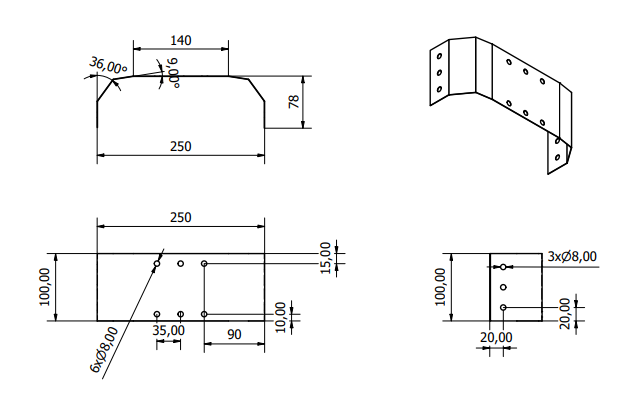
\includegraphics[scale = 0.9]{Figures/NewFrontDWG.png}
    \caption{Platform Front and Back Design}
    \label{fig:newfrontdwg}
\end{figure}

\begin{figure}[H]
    \centering
    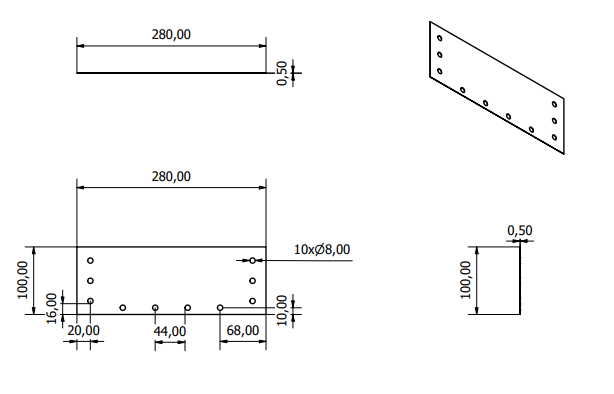
\includegraphics[scale = 0.9]{Figures/NewSideDWG.png}
    \caption{Platform Side Design}
    \label{fig:newsidedwg}
\end{figure}

\begin{figure}[H]
    \centering
    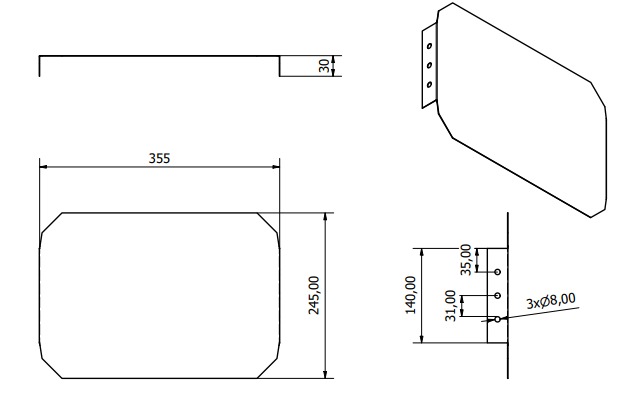
\includegraphics[scale = 0.9]{Figures/NewTopDWG.png}
    \caption{Platform Top Design}
    \label{fig:newtopdwg}
\end{figure}

Figure \ref{fig:newfrontdwg} represents the front and the back of the platform while figure \ref{fig:newsidedwg} represents the sides of the platform. Figure \ref{fig:newtopdwg} shows the design for the top of the platform. This part will hold the payload. The dimensions were selected to ensure the platform meets the maximum size of 450mm in length, width and height as set out in the design considerations. 

The final platform design is as shown in figure \ref{fig:platformdesign}.

\begin{figure}[H]
    \centering
    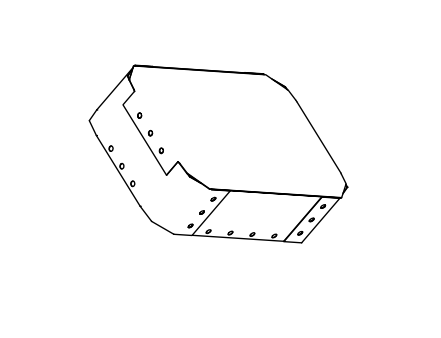
\includegraphics{Figures/bodyParts.png}
    \caption{Platform Assembly}
    \label{fig:platformdesign}
\end{figure}


\subsubsection{Fabrication}
Fabrication of the different parts of the platform body involved various sheet metal operations, including cutting, bending, drilling and joining. From the design considerations in \ref{sec:bodydesign}, the primary material selected for fabrication was aluminium. However, several challenges emerged when it came to the acquisition, that is:
\begin{enumerate}[i.]
    \item Aluminium was difficult to find, especially in local shops. Consequently, online international shops had to be considered, but due to time constraints, they were considered unrealistic sources.
    \item Aluminium was expensive compared to other materials such as mild steel and galvanized steel. Most retailers listed aluminium at three times the price of mild steel.
    \item Retailers further sold the material in large proportions which would mean a lot of waste material once the fabrication was done. This made little financial sense in the long run.
\end{enumerate}

Due to these challenges, aluminium was disregarded as the material of choice. Mild steel was the best alternative mainly due to the fact that it is readily available and relatively cheap to acquire. Furthermore, cost sharing was a real possibility due to most projects having mild steel as their material of choice.
\vspace{2mm}

Once the material was acquired, the next step was machining. The first step was cutting the sheet metal into the design dimensions. For instance, the platform side part was cut into two $280mm$ by $100mm$ pieces, whereas the front was cut into two $360mm$ by $100mm$ pieces and the top part was cut into a $355mm$ by $245mm$ piece. This was achieved using a hydraulic shearing machine.

\vspace{3mm}
The next step was bending the platform front parts (Figure \ref{fig:newfrontdwg})
The folding angles were $9^0$, $36^0$ and $45^0$. That precise order was followed to produce the desired shape on a manual bending machine. However, there were several limitations to this process, given that measuring the angles during bending was impossible. This meant approximations had to be made by eye during the process and confirmed later using a protractor. This might have resulted in some inaccurate angles but tolerances had been accounted for in the design process. The platform top (Figure \ref{fig:newtopdwg}) was also  machined to create the $45^0$ bend on either of its ends.


The final step in sheet fabrication was joining. Several joining methods were considered in the design process, including welding, screws and riveting. However, the two best were determined to be spot welding and using machine screws and nuts. To accommodate the machine screws, holes had to be created on the sheet metals. Diameter $3mm$ screws and nuts were the sizes selected. The holes were created using a drilling machine and $3mm$ drill bits. The holes were made on the bottom part of the platform side (Figure \ref{fig:newsidedwg}) and the bottom part of the platform front (Figure \ref{fig:newfrontdwg}). These holes would be used to join the platform body to the chassis.

\vspace{3mm}
The platform side and front were joined using spot welding. To carry out the spot weld, the surfaces had to be cleared of all stains and roughness. An emery paper was used to achieve a smooth and shiny surface on all the surfaces that would be used for joining. 

The platform top was joined to the other parts using machine screws and nuts. This fulfilled a design consideration in Section \ref{sec:bodydesign} as it made the design easy to assemble and disassemble.

\begin{figure}[H]
    \centering
    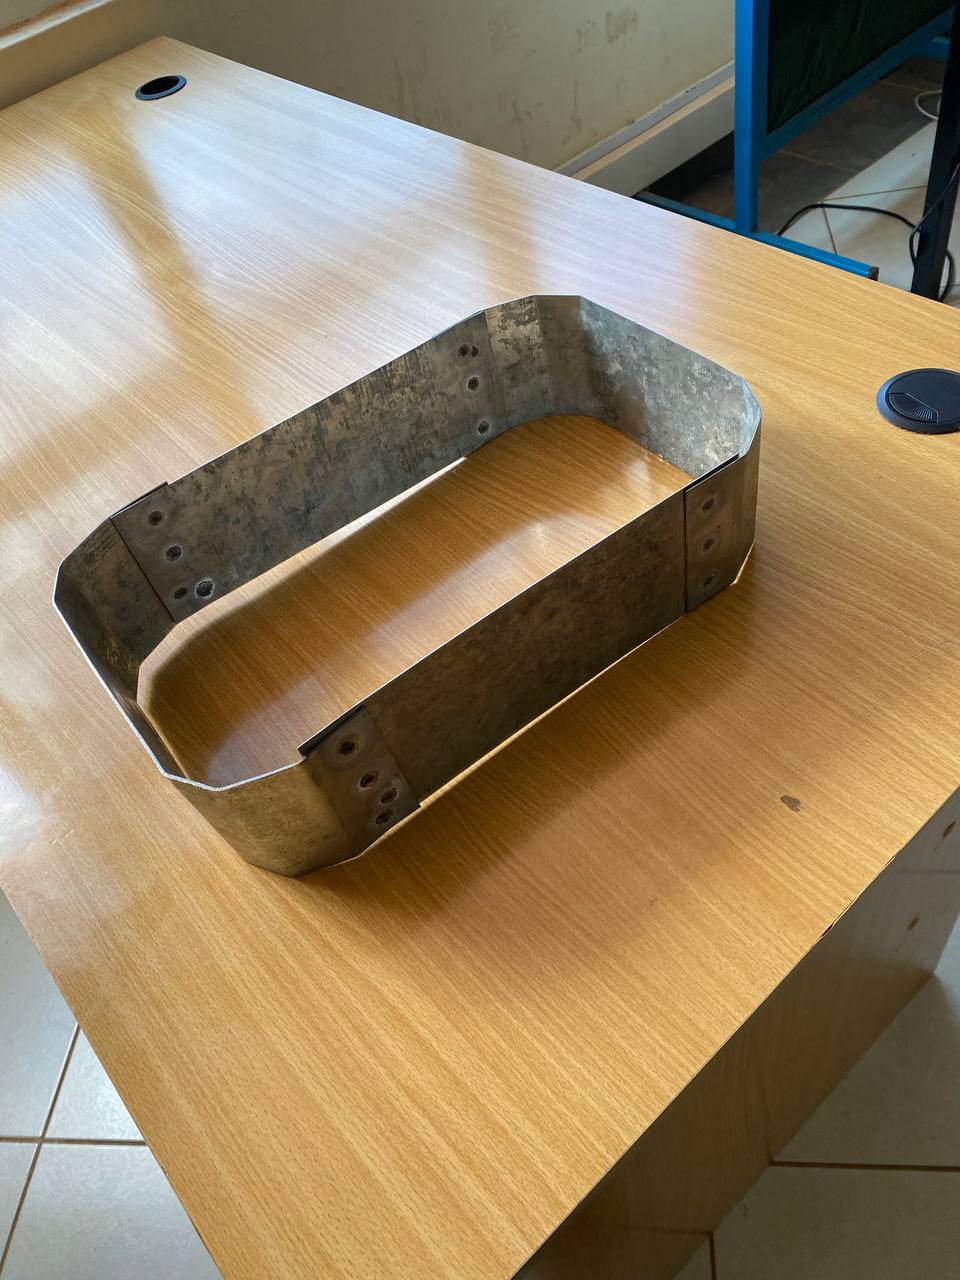
\includegraphics[scale = 0.2]{Figures/platformBodyFAB.jpg}
    \caption{Front and side assembly}
    \label{fig:platformBFAB}
\end{figure}

\begin{figure}[H]
    \centering
    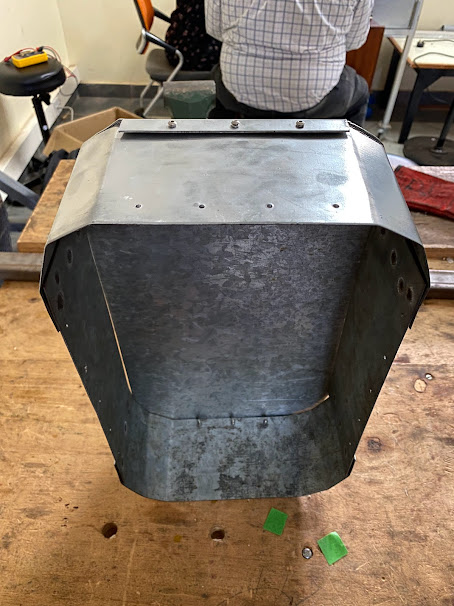
\includegraphics[scale = 0.35]{Figures/bodyFABRICATEDfront.jpg}
    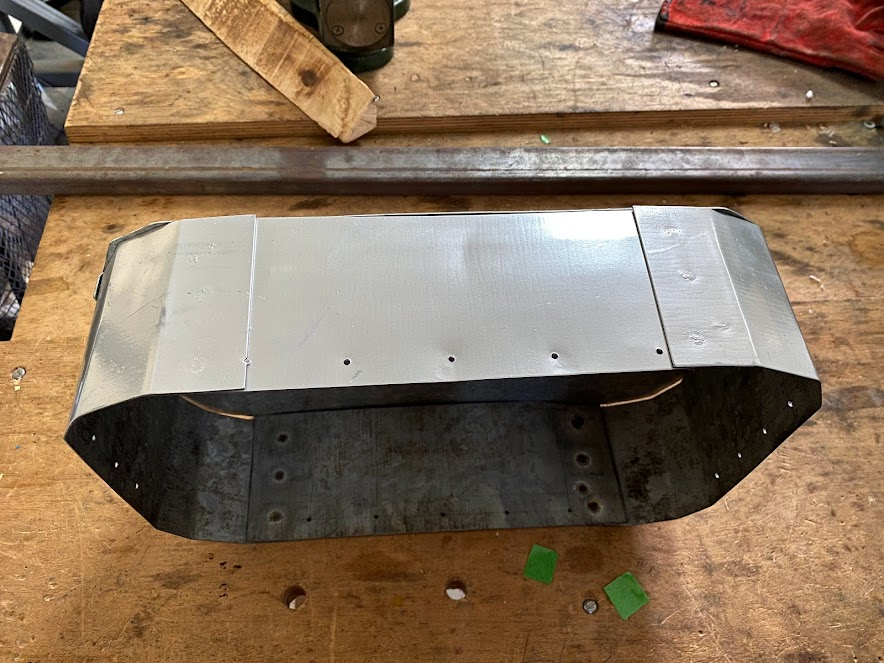
\includegraphics[scale = 0.30]{Figures/bodyFABRICATEDside.jpg}
    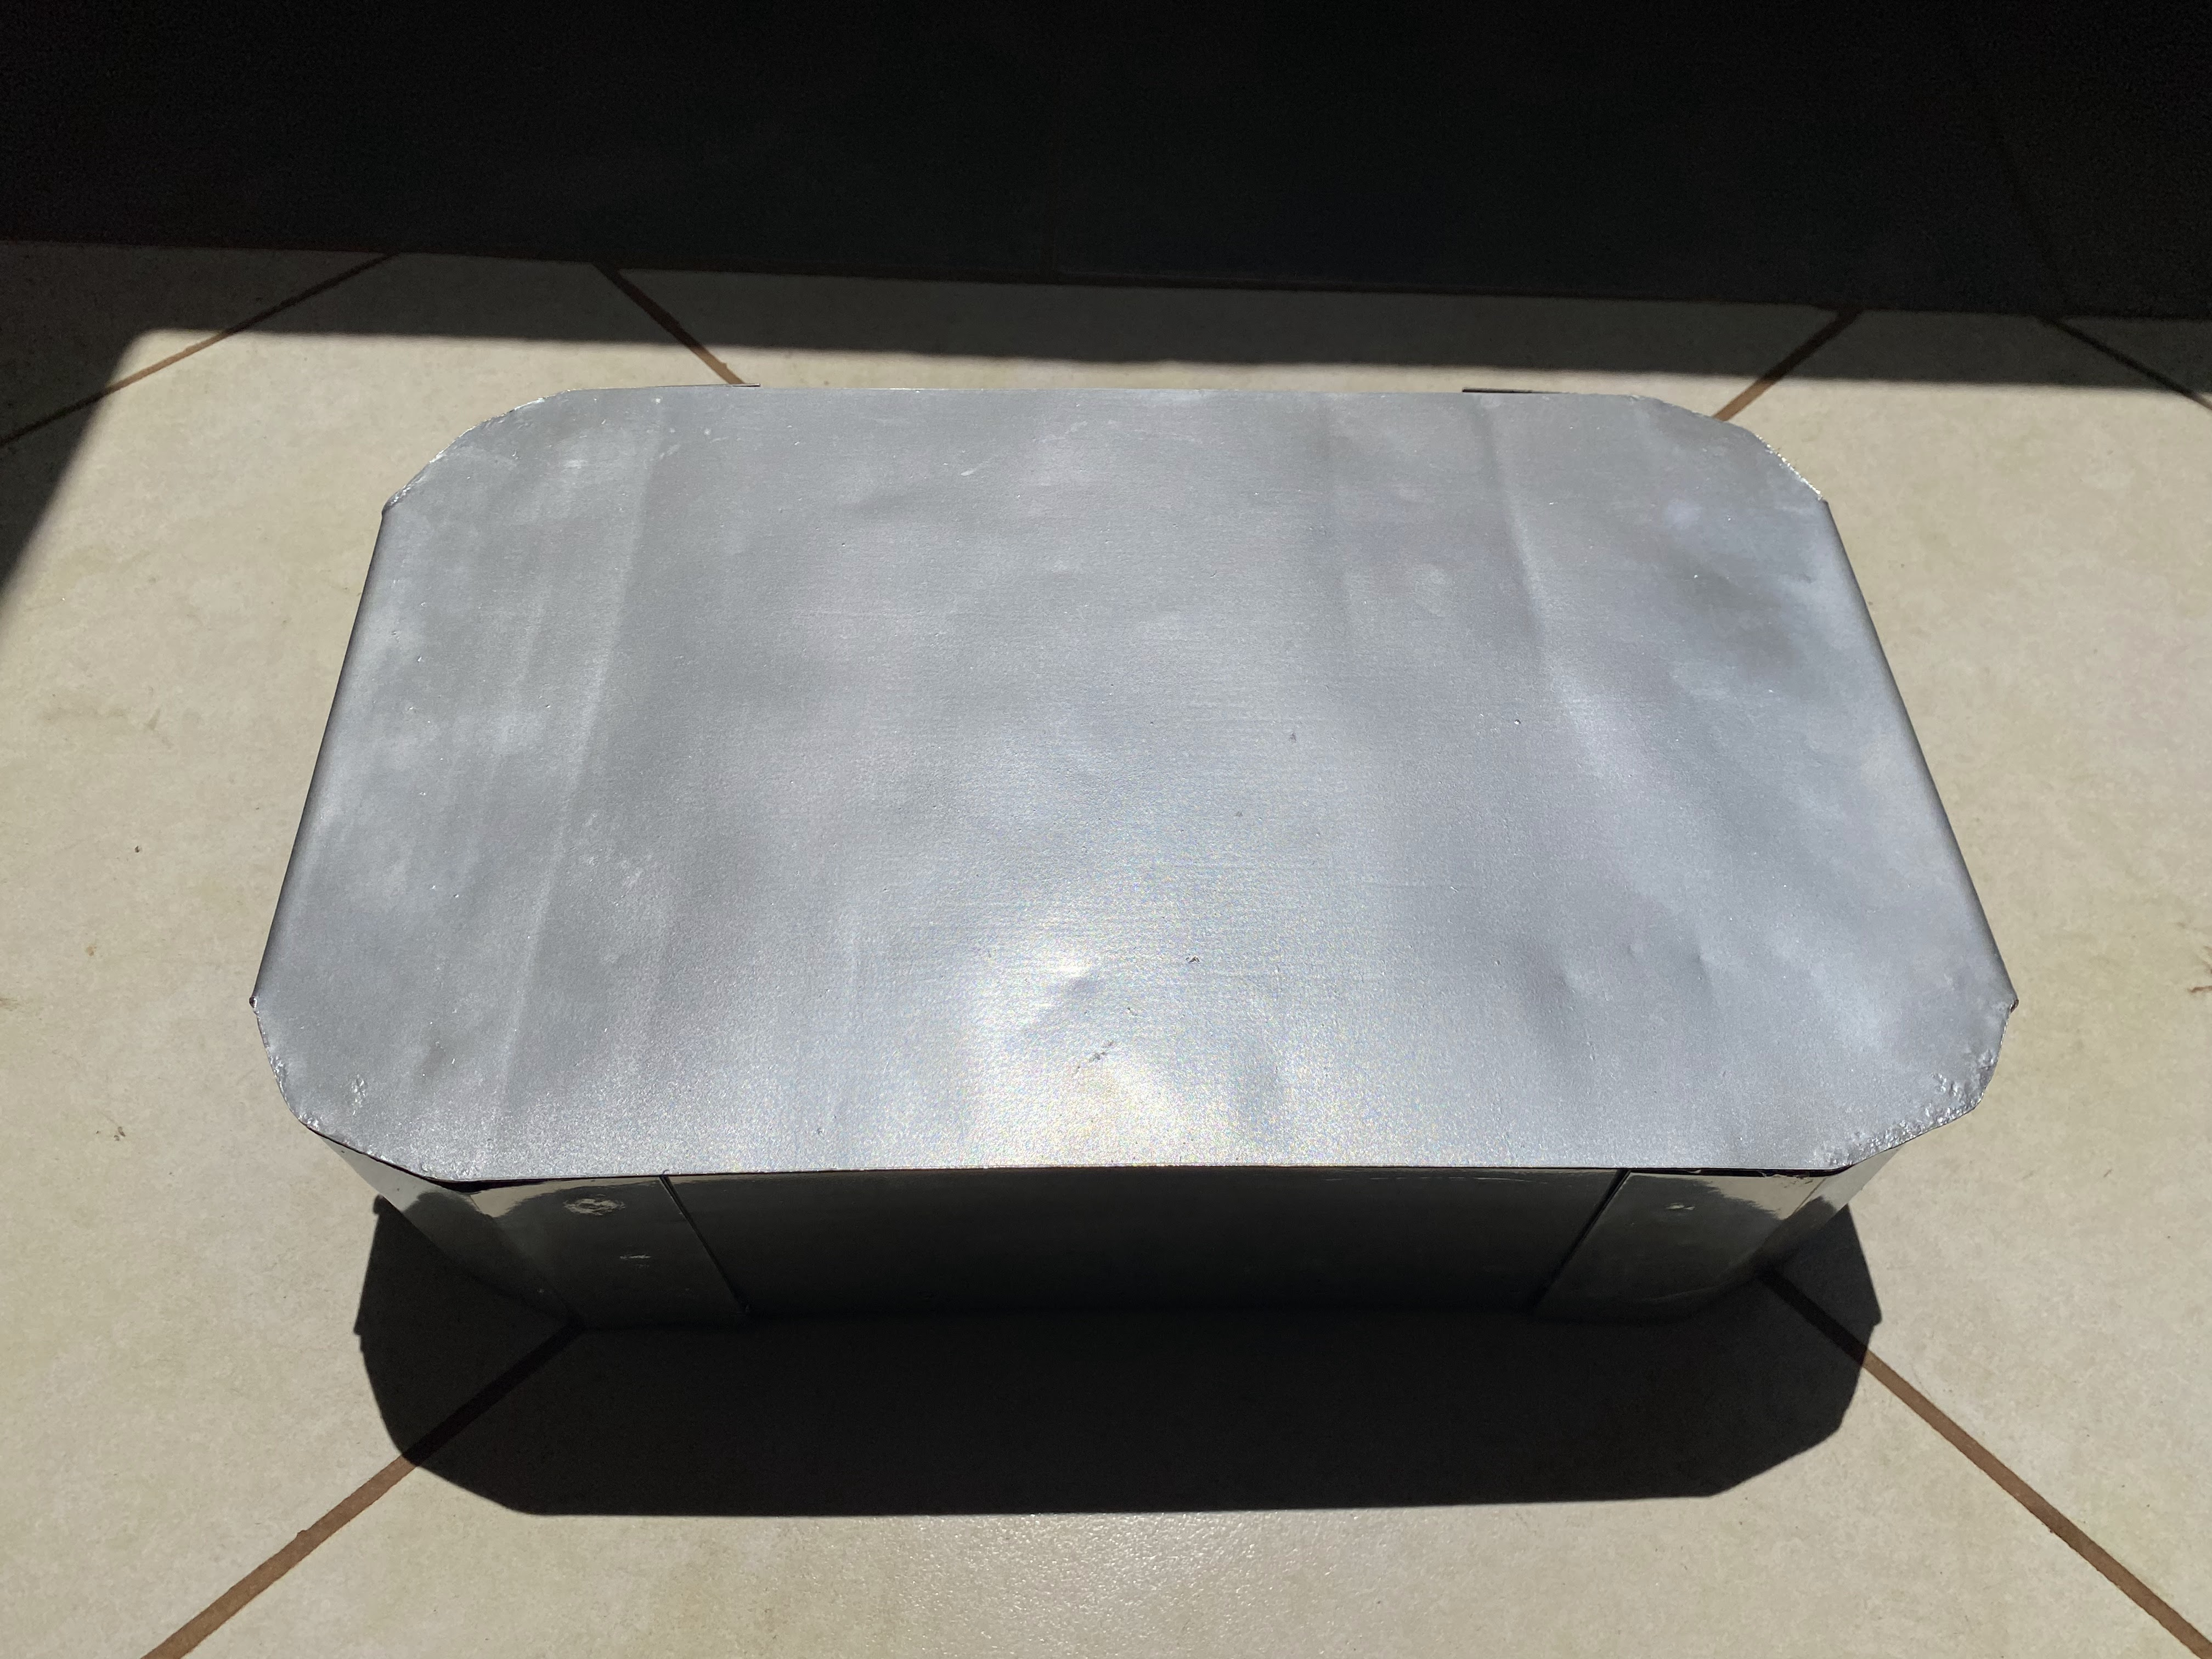
\includegraphics[scale = 0.1]{Figures/bodyFABRICATEDtop.jpg}
    \caption{Fabricated Platform Body}
    \label{fig:fabPlatf}
\end{figure}

\subsection{Platform Chassis}
\subsubsection{Design}
The design considerations made for the platform chassis were:
\begin{enumerate}[i.]
    \item Load capacity
    \item Material selection
    \item Chassis type
\end{enumerate}

The first two considerations are directly related as it was important to select the chassis material based on its ability to handle a payload, a factor determined by the tensile strength, compressive strength, and torsional strength. The chassis carries the whole load and therefore the material selected needed to have high tensile strength. Table \ref{table:materialproperties} was used to make this determination and mild steel was settled on as the material of choice. Stainless steel was considered but material cost was a huge factor in the design process.
\par
There are many types of chassis designs each suited to handle the load cases described above. There are ladder frames that carry all load and have good bending strength and stiffness. Other types are cruciform frames which can carry torsional loads. They are made of two straight beams and have only bending loads. The torque tube backbone (tube-frame) frame is made of a closed box section as the main backbone. Traverse beams resist lateral loads and backbone frame bending and torsion. 
\par
Considering all these properties, it was determined that a blend of cruciform frames and traverse beams would be ideal to accommodate all forces. The developed chassis design is as shown by figure \ref{fig:newchassis}. These designs were made using Autodesk Inventor 3-D modelling software.

\begin{figure}[H]
    \centering
    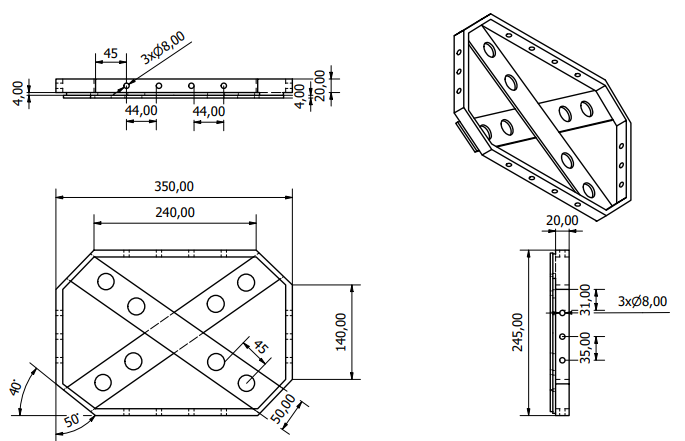
\includegraphics[scale = 0.8]{Figures/NewChassisDWG.png}
    \caption{Chassis Design}
    \label{fig:newchassis}
\end{figure}

\subsubsection{Fabrication}
\label{sec:chassisFAB}
The material selected for use was rectangular mild steel bars with a $2mm$ thickness and $20mm$ width. Several processes needed to be carried out to come up with the design in Figure \ref{fig:newchassis}, including marking, cutting, filing, drilling and joining.
Some of the tools and equipment required to do this include: 
\begin{enumerate}[i.]
    \item steel rule
    \item scriber
    \item file
    \item hacksaw
    \item hydraulic shearing machine
    \item drilling machine
    \item drill bits
    \item arc welding machine
\end{enumerate}

First, the general length dimensions were marked out and four bars were produced by cutting the raw material on a hydraulic shearing machine. The lengths of these bars were $240mm$ and $140mm$, two of each. Four smaller bars that would join the front and side bars were cut using a hacksaw because of their relatively small lengths. 
Two more bars that would form the diagonals to form some form of cruciform were cut separately with dimensions of $50mm$ width and $350mm$ length. 
\par
All the holes were then made on the drilling machine. Holes were made on the diagonal metal bars using an $8mm$ drill bit and would be used to attach the wheels and motors to the chassis. The front and side bars were also drilled using $3mm$ drill bits for assembly to the platform body in Figure \ref{fig:platformBFAB}
\par
Once all the individual parts were fabricated, they were all joined using metal arc welding, a fusion welding process used to join metals. They were joined as depicted in Figure \ref{fig:newchassis} and Figure \ref{fig:chassisFAB}
\par
Figure \ref{fig:chassisFAB} is a visual representation of the results of the chassis fabrication process.

\begin{figure}[H]
    \centering
    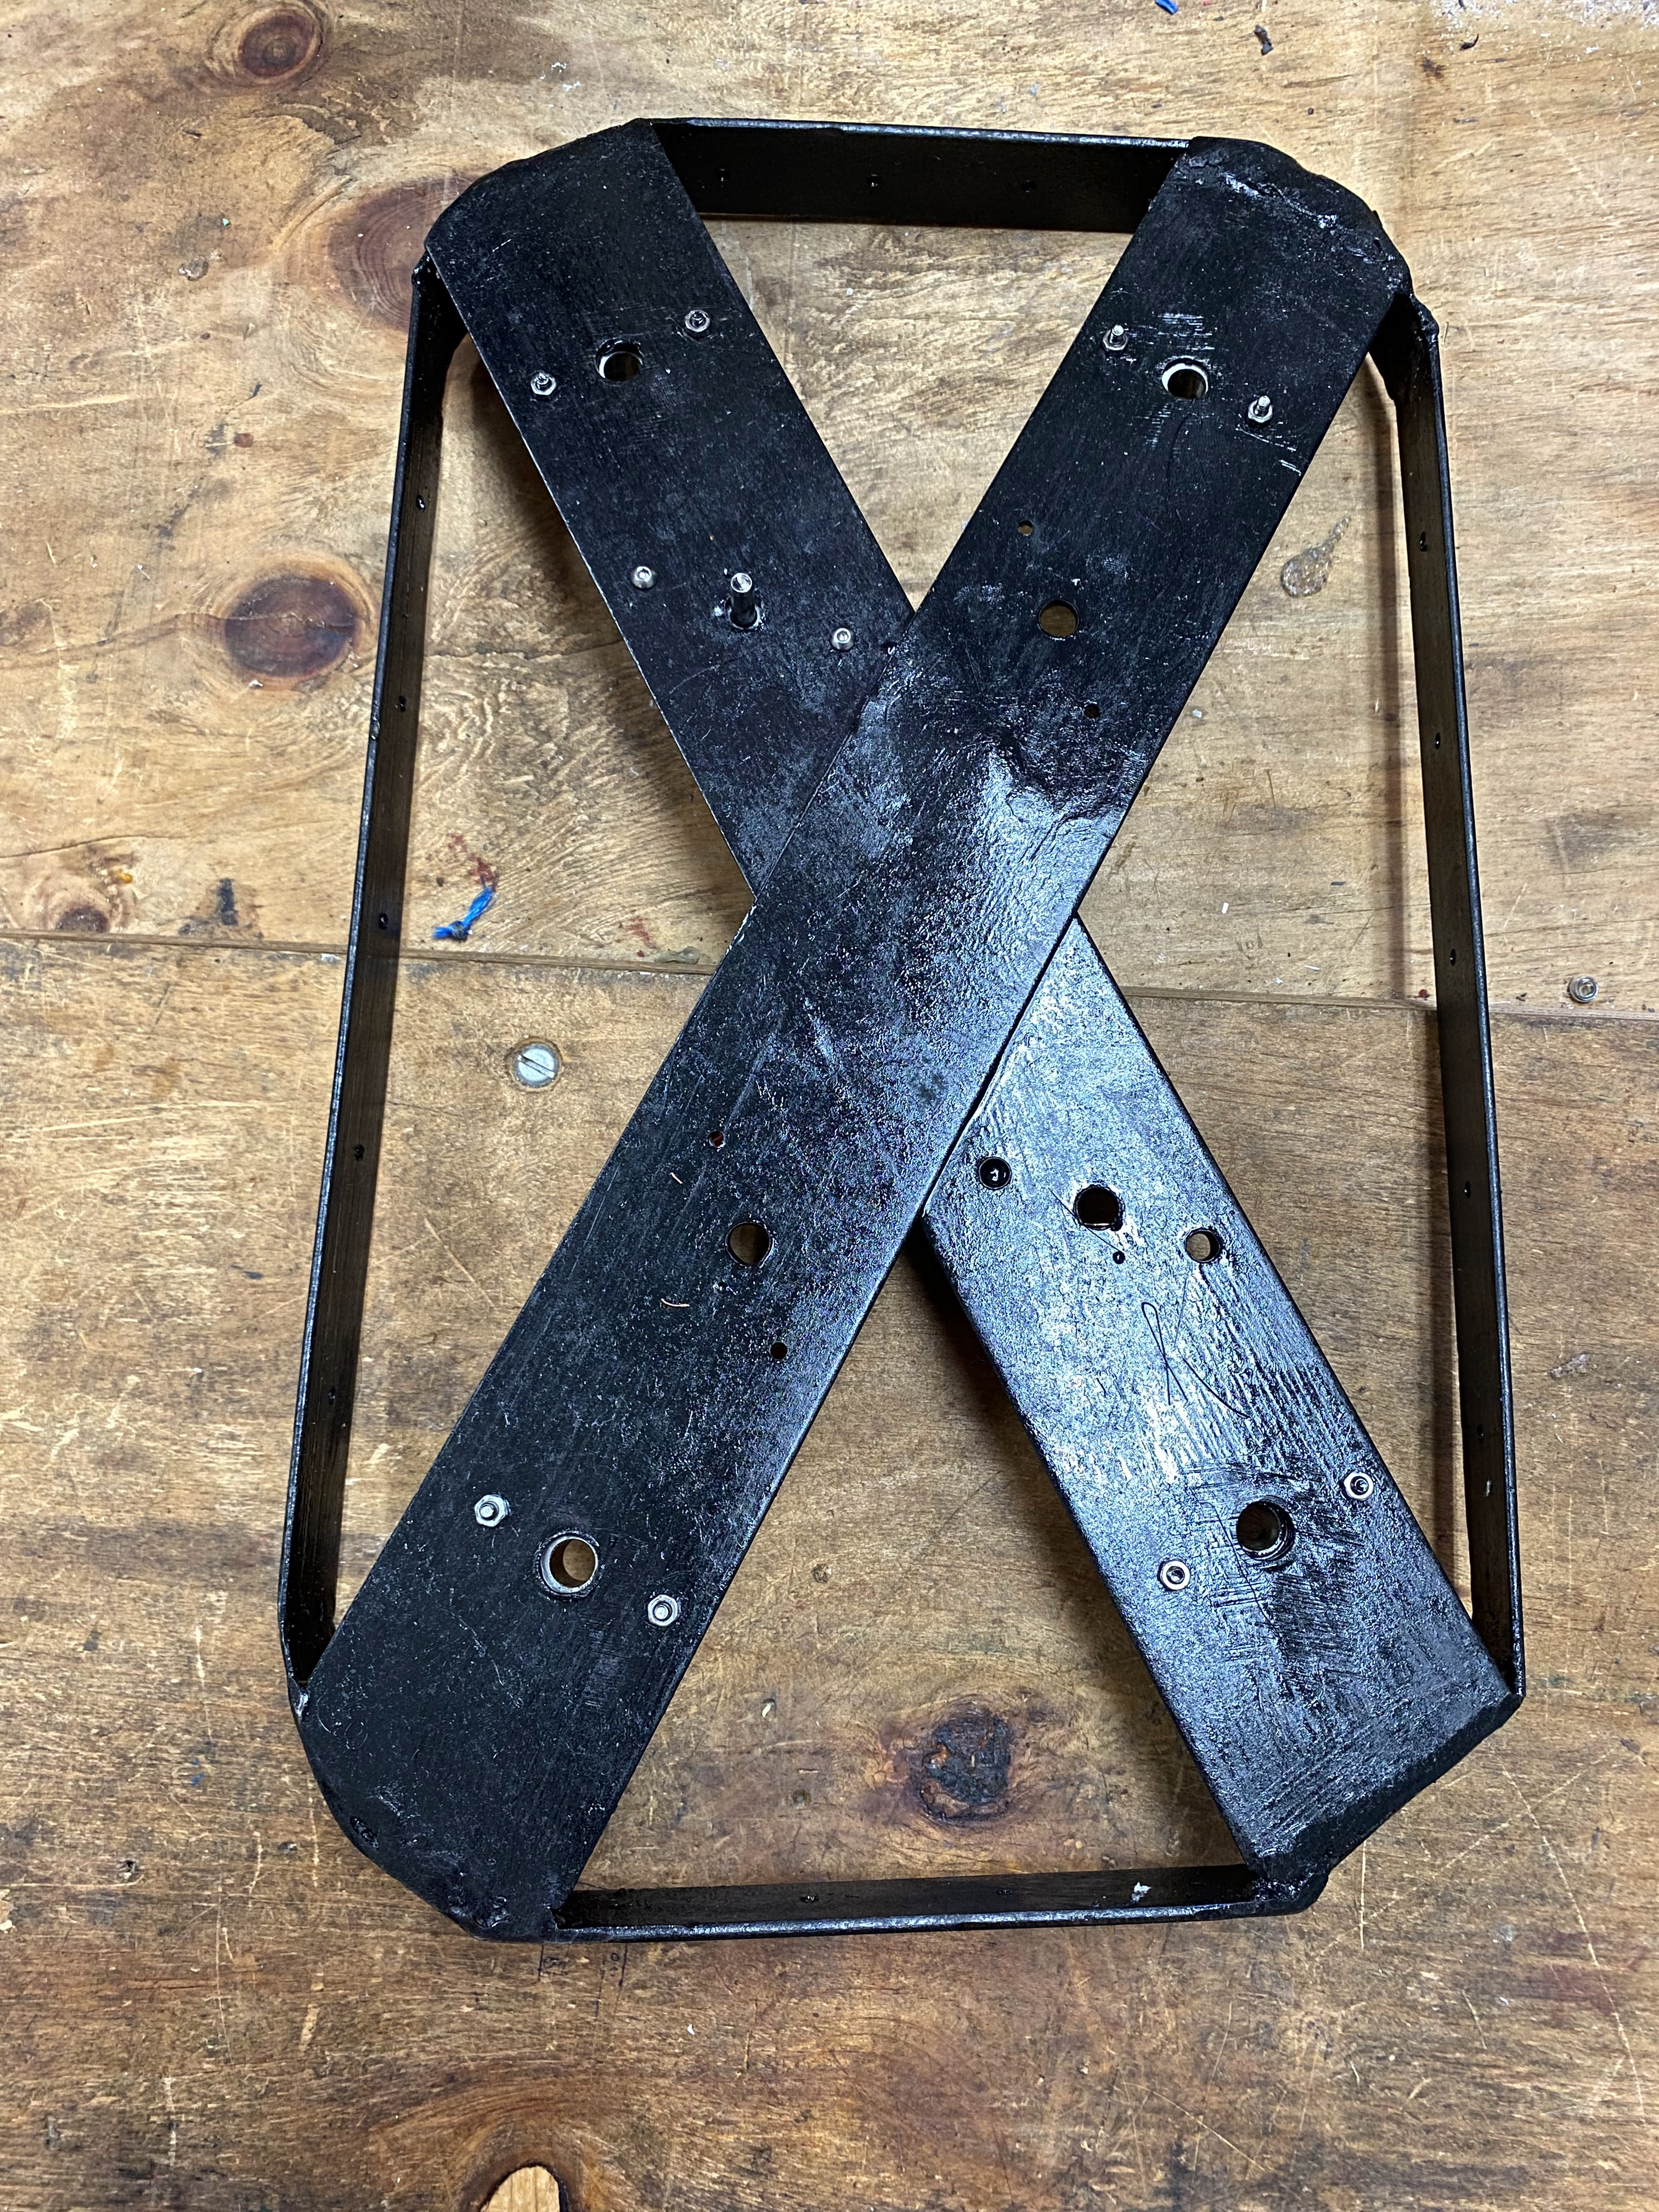
\includegraphics[scale = 0.10]{Figures/chassisFABRICATED.jpg}
    \caption{Chassis}
    \label{fig:chassisFAB}
\end{figure}

\subsection{Wheel Frame}
\subsubsection{Design}
\label{sec:wheelDesign}

The wheel frame had similar payload design considerations as the chassis because the frame would be supporting all the weight from the platform. The frame would handle the bulk of the load and therefore a high tensile and
yield strength material would be required. Mild steel was the go-to material for the chassis and would be here as well. Other considerations would be the size since it would hold the caster wheel, drive \ac{DC} motor, and the power transmission system. The most common \ac{DC} motors have diameters ranging between $25mm$ and $30mm$ while their lengths range between $40mm$ and $70mm$. The motor selected had a diameter of $25mm$ and a total length of $45mm$. Section \ref{sec:motor} provides more information on motor selection. The power transmission system of choice would be a belt and pulley of a maximum diameter of $16mm$. The caster wheel of choice had a diameter of $70mm$. 
\par
Taking all these dimensions and parameters into consideration, the dimensions of the wheel frame were determined to be a height of $90mm$, length of $50mm$, and width of $50mm$ as in Figure \ref{fig:newframe}.

\begin{figure}[H]
    \centering
    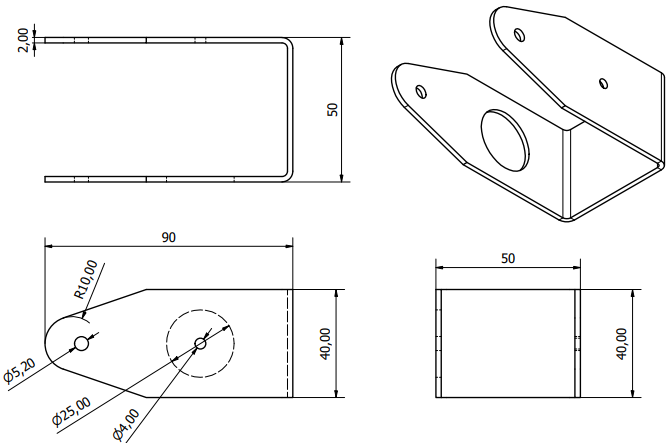
\includegraphics[scale = 0.8]{Figures/NewFrameDWG.png}
    \caption{Wheel Frame Design}
    \label{fig:newframe}
\end{figure}

\subsubsection{Fabrication}
The wheel frame material used was similar to the material used to fabricate the platform body in Figure \ref{fig:platformBFAB}. A mild steel metal sheet of thickness $1.5mm$ was machined to produce the frame by going through processes such as cutting, bending, drilling and filling.
\par
The first operation was cutting the wheel frame to a length of $230mm$ and width of $40mm$ using the hydraulic shearing machine. Next, various holes that would hold bearings and the motor were made using a drilling machine. The bearing holes were made using $10mm$ drill bits while the motor holes were made using $25mm$ drill bits. However, to make the $25mm$ hole, several drill bits were used to offset the torque generated by the drilling machines. This consideration was made due to one of the wheel frames getting destroyed by a $25mm$ drill bit due to high torque and a large drill bit diameter as in Figure \ref{fig:frameBAD}. 

\begin{figure}[H]
    \centering
    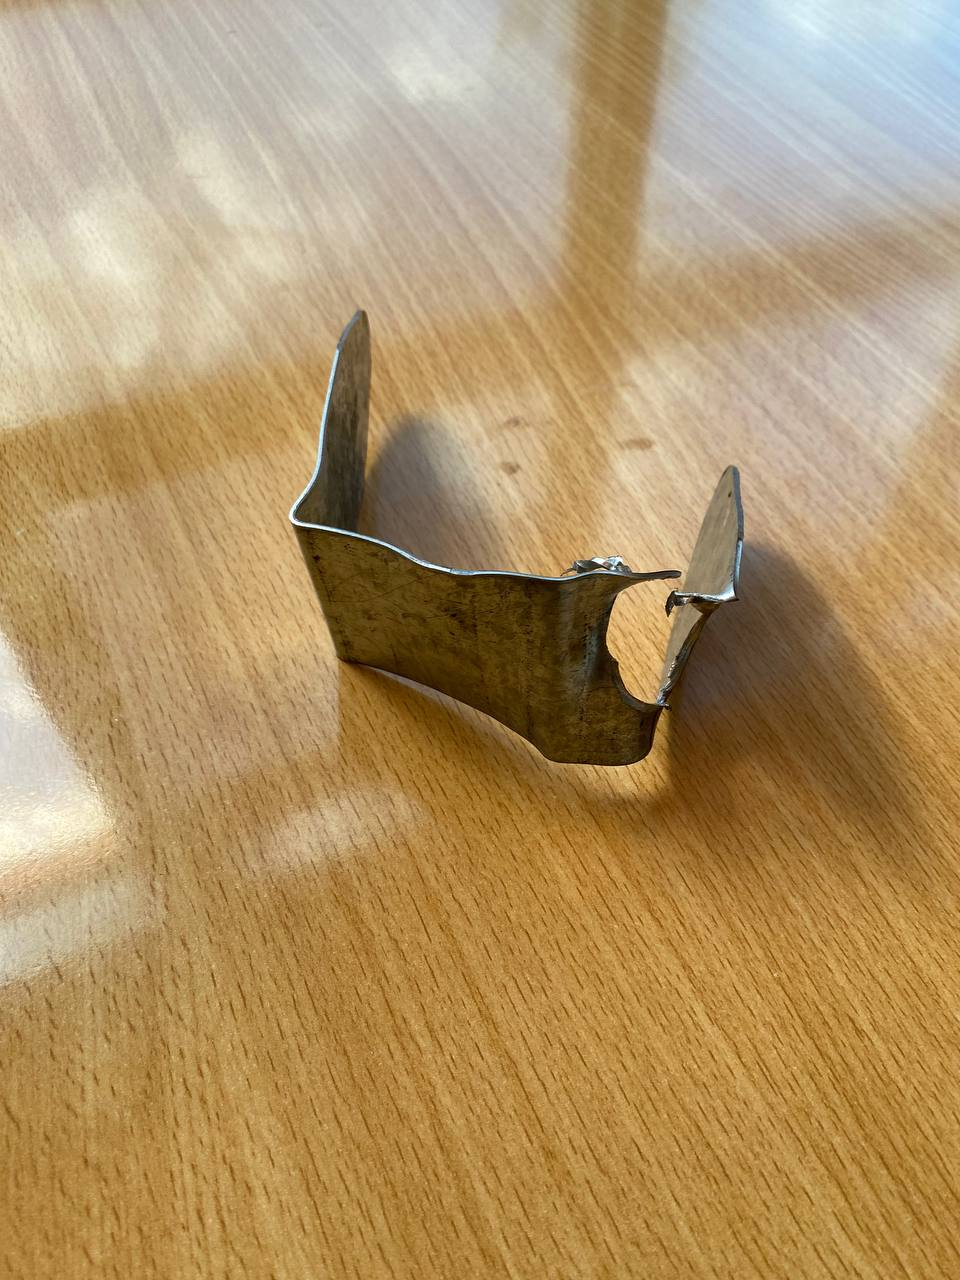
\includegraphics[scale = 0.3]{Figures/frameBAD.jpg}
    \caption{Wheel Frame Fabrication Challenge}
    \label{fig:frameBAD}
\end{figure}

\par
The next step was filing the wheel frame to achieve the angled shape at either end of the wheel frame. Finally, the frame was bent as in Figure \ref{fig:frameFAB} using a manual bending machine to create $90^0$ bends, to give the final result.

\begin{figure}[H]
    \centering
    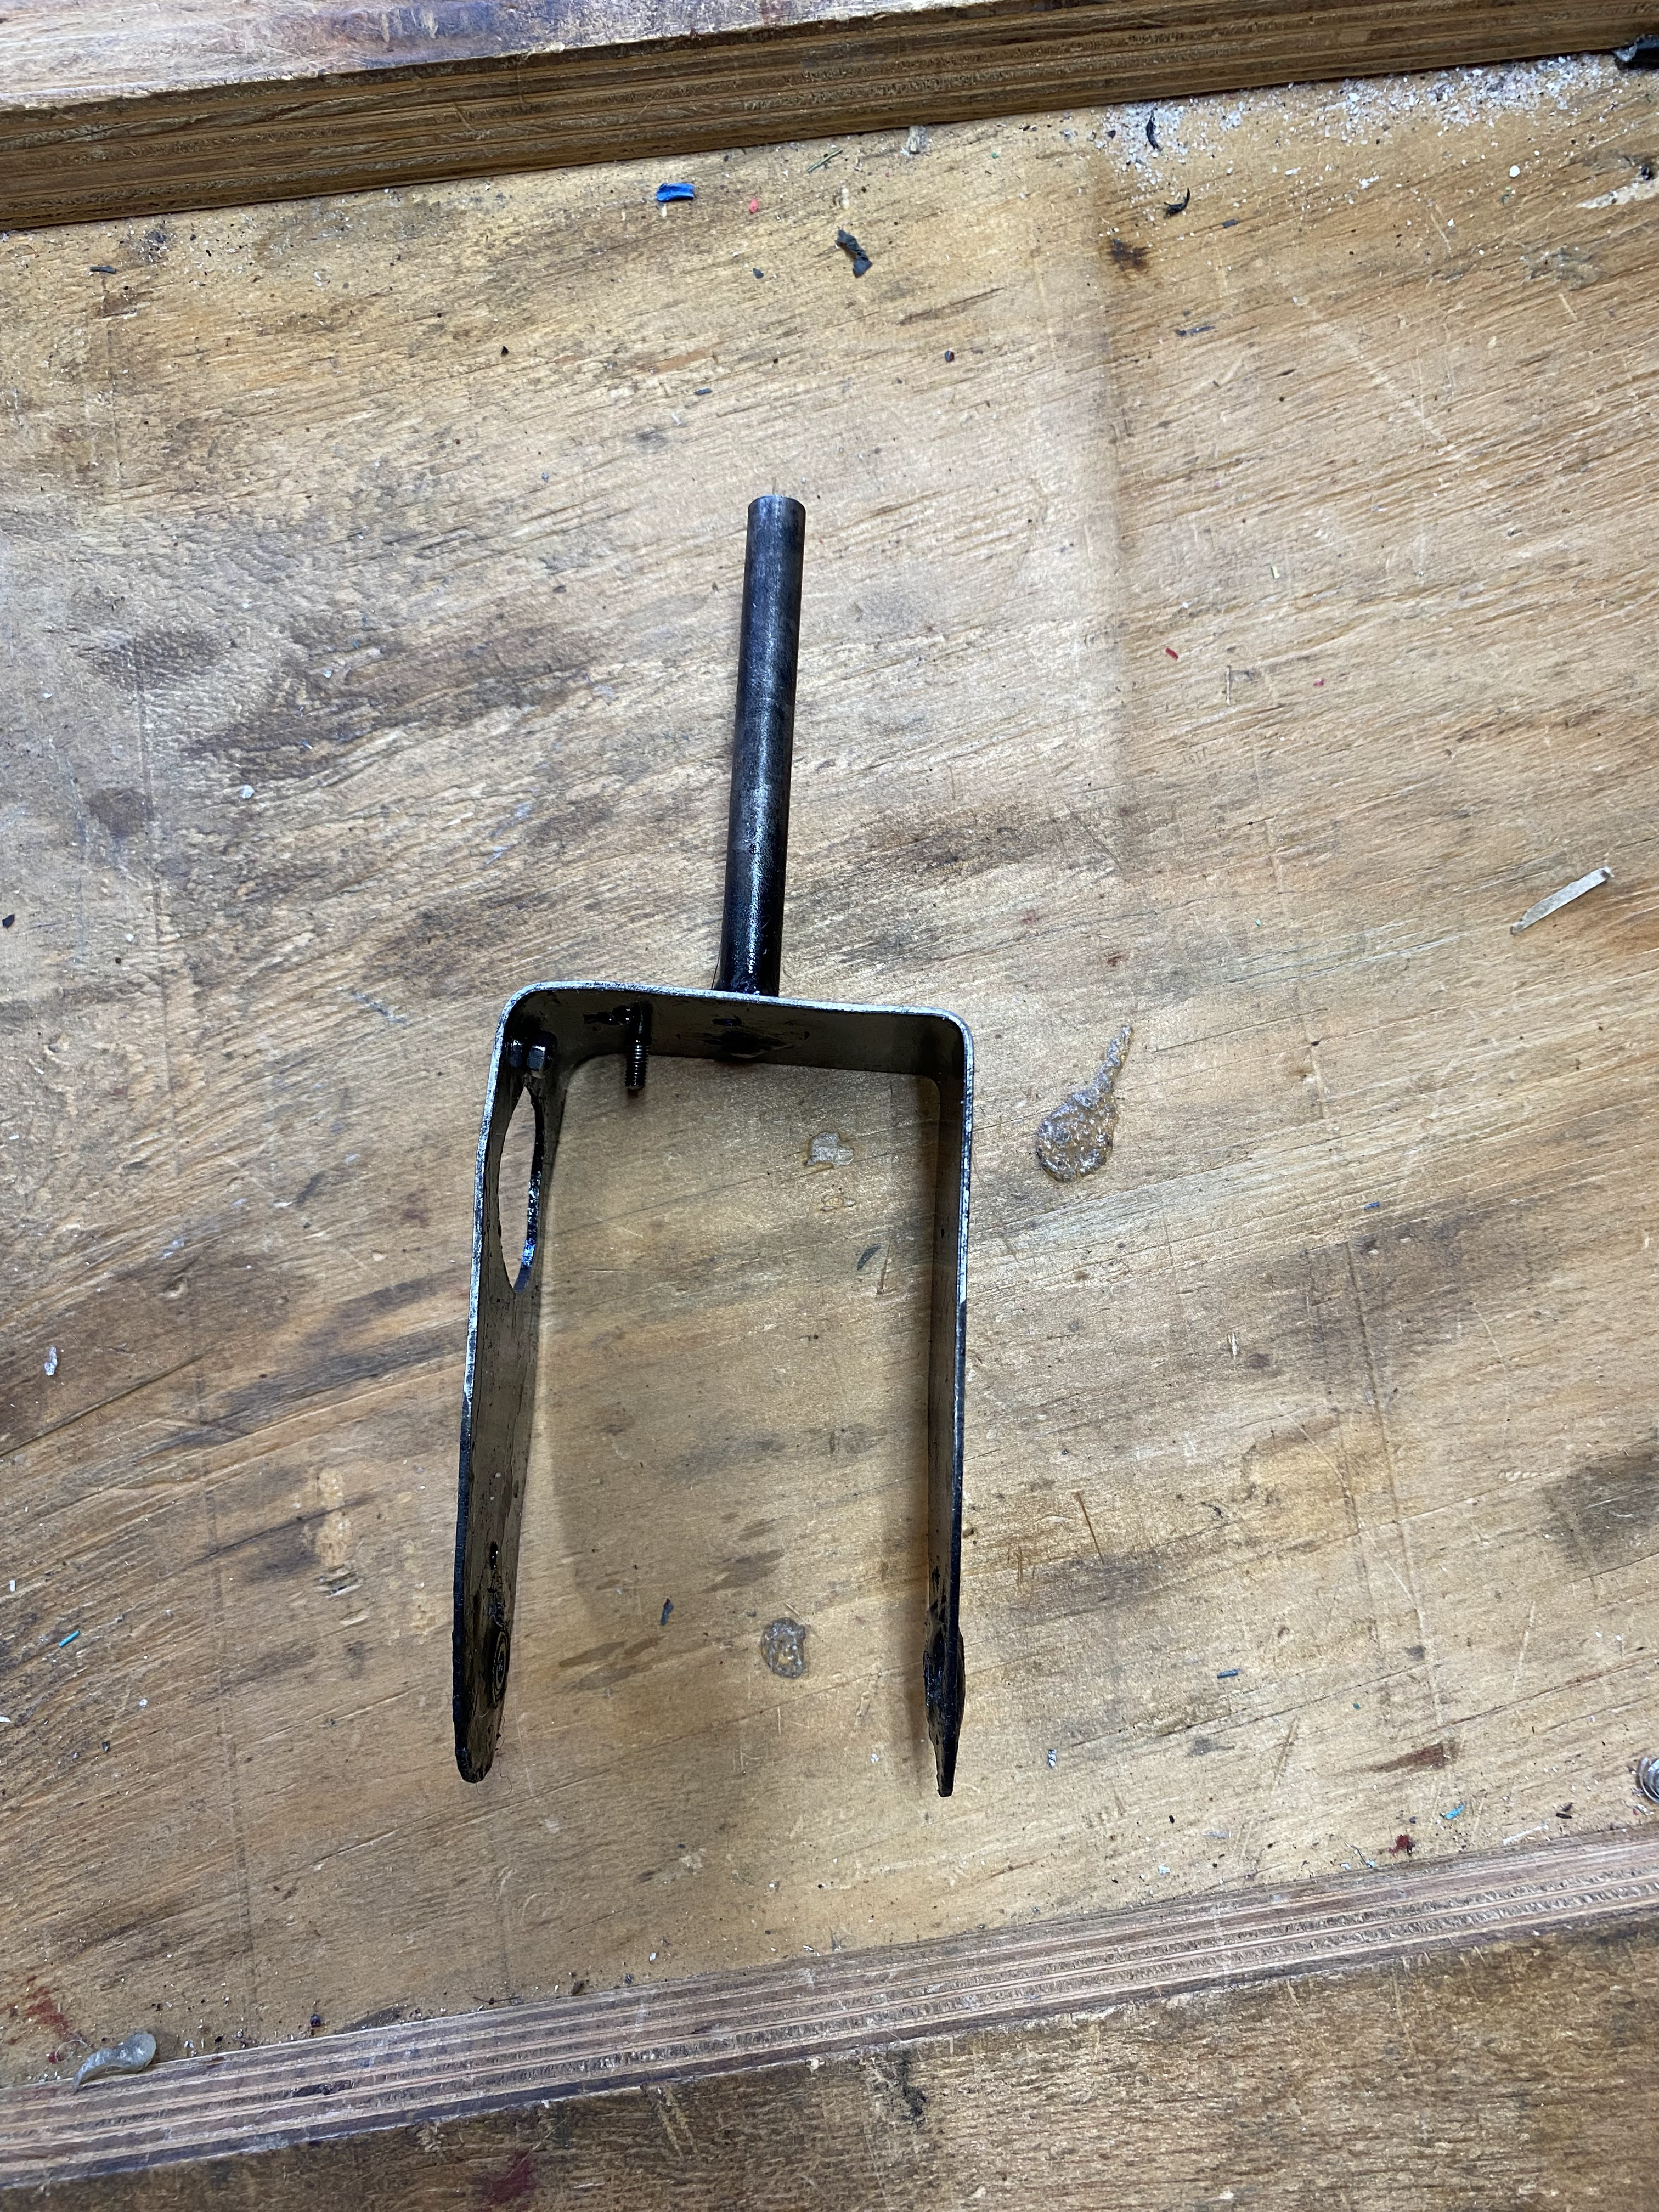
\includegraphics[scale = 0.07]{Figures/wheelFRAMEempty1.jpg}
    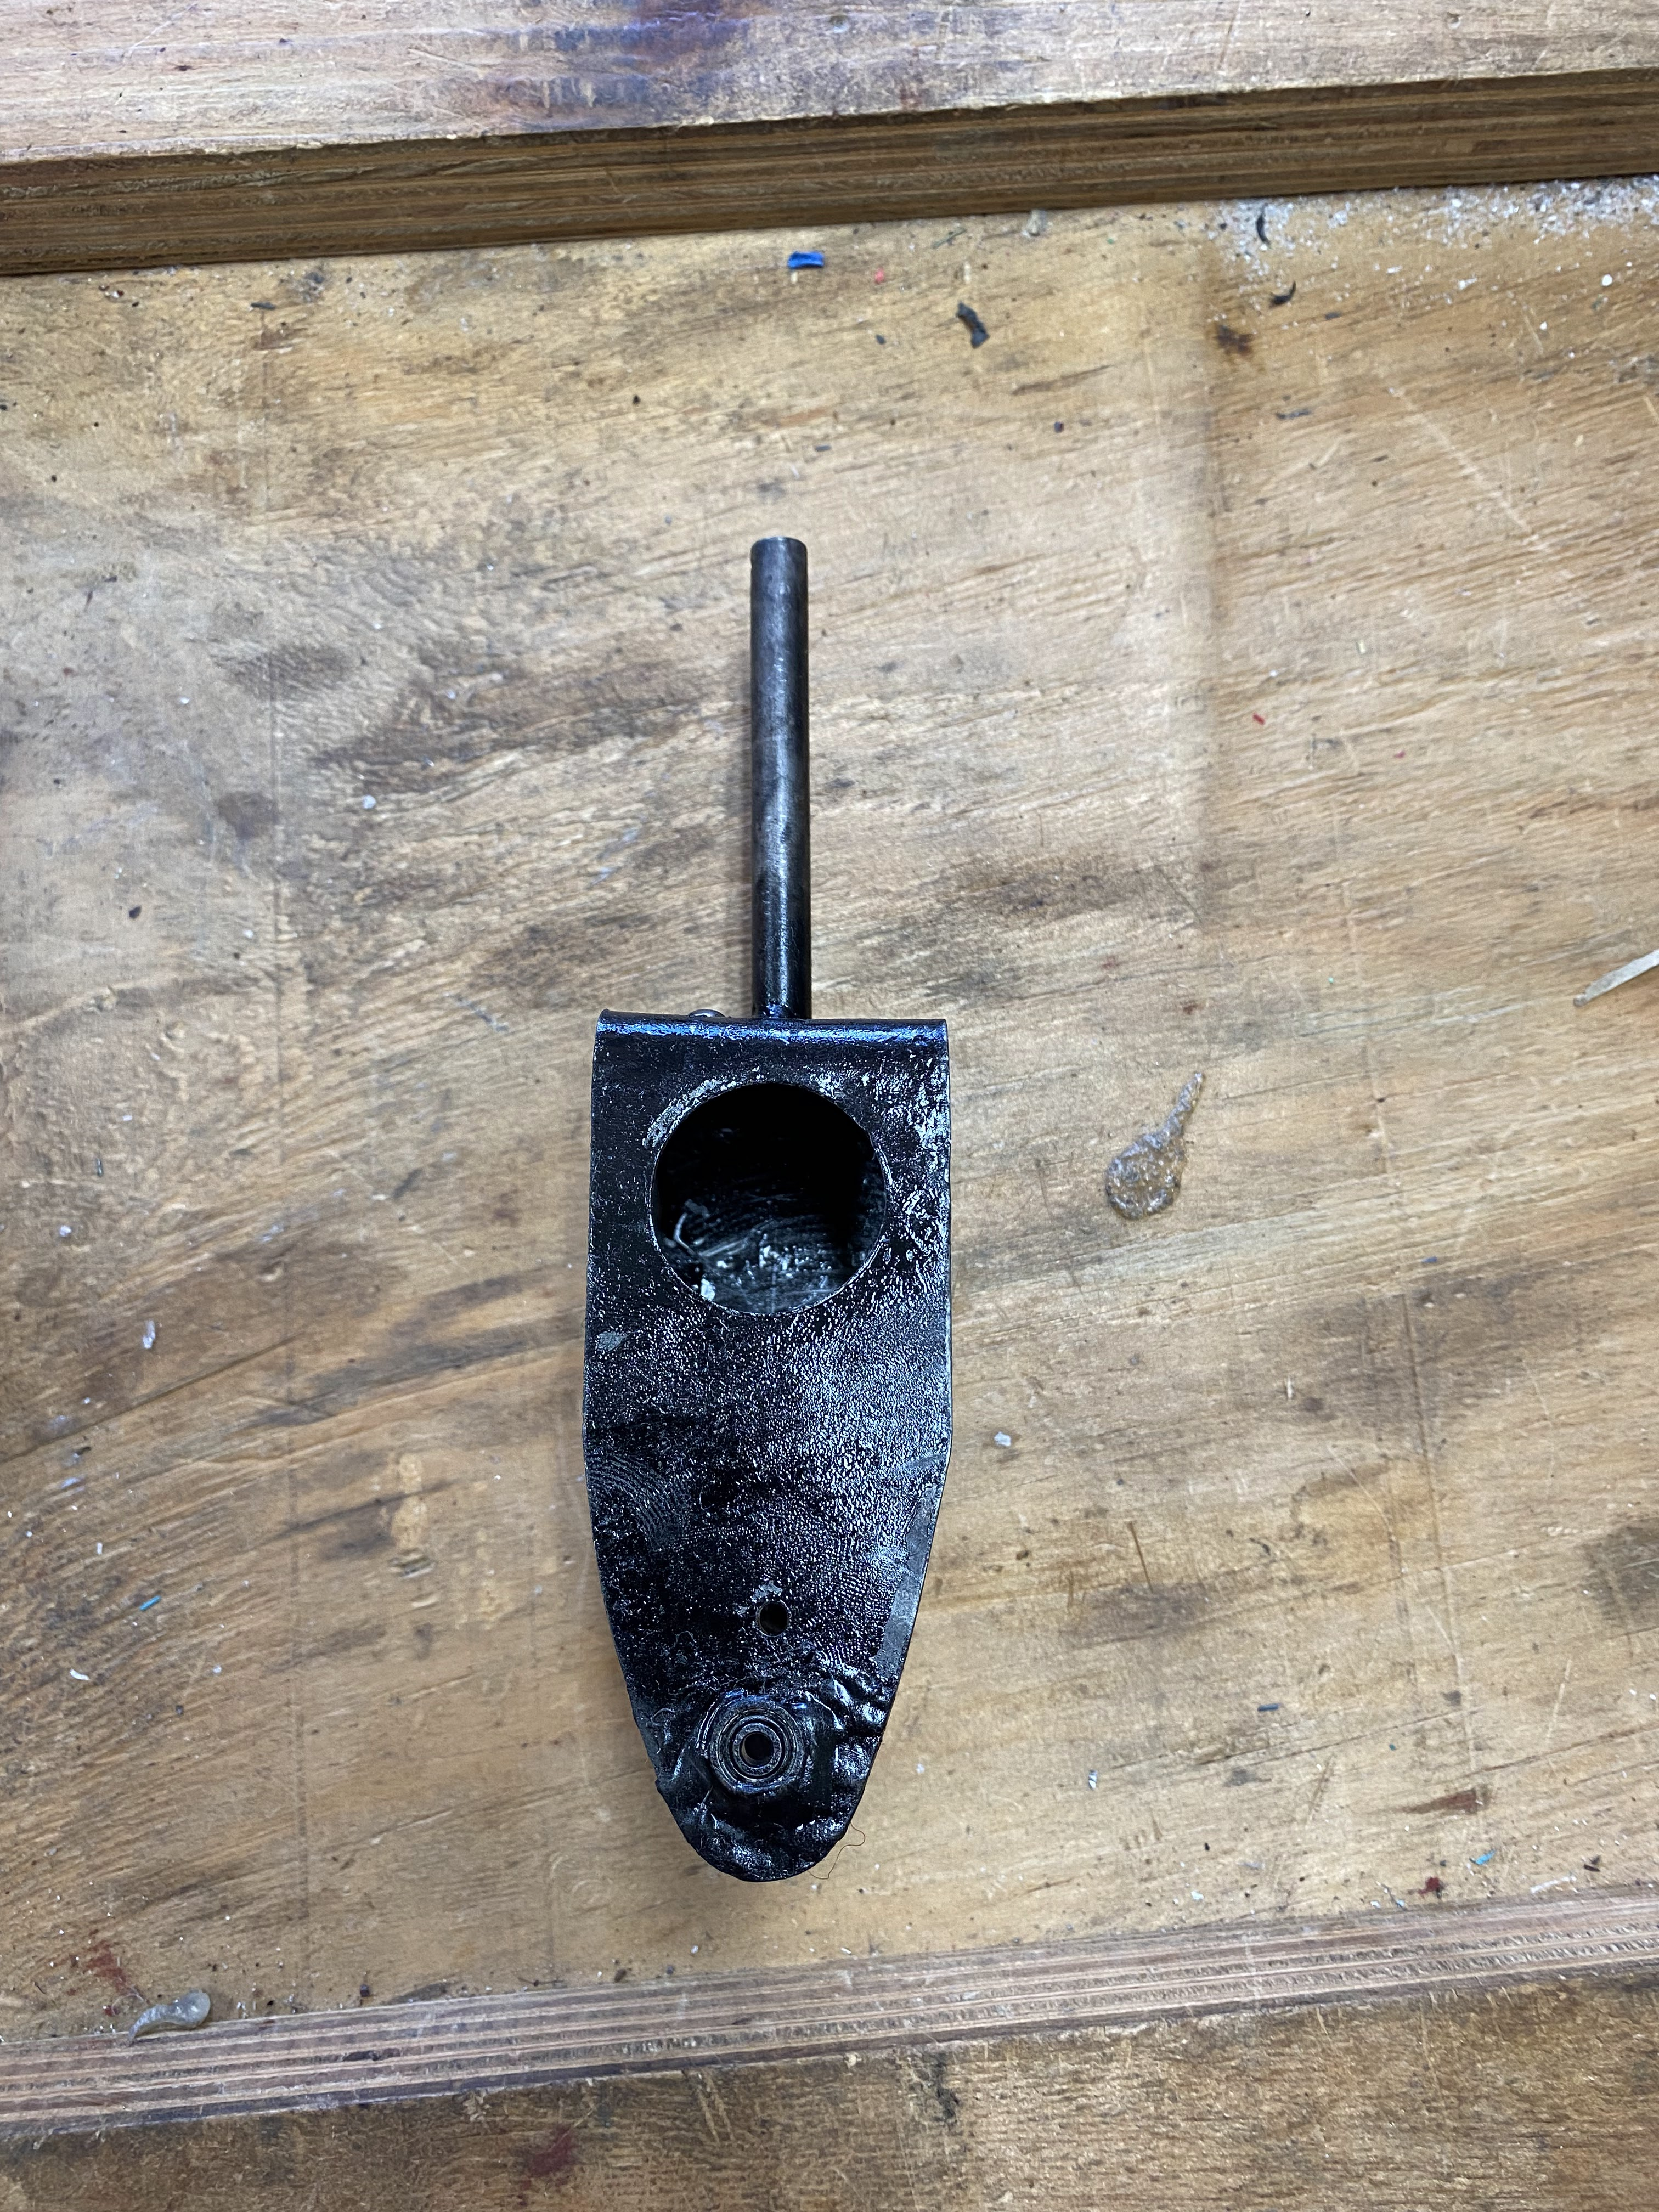
\includegraphics[scale = 0.07]{Figures/wheelFRAMEempty2.jpg}
    \caption{Wheel Frame}
    \label{fig:frameFAB}
\end{figure}

\begin{figure}[H]
    \centering
    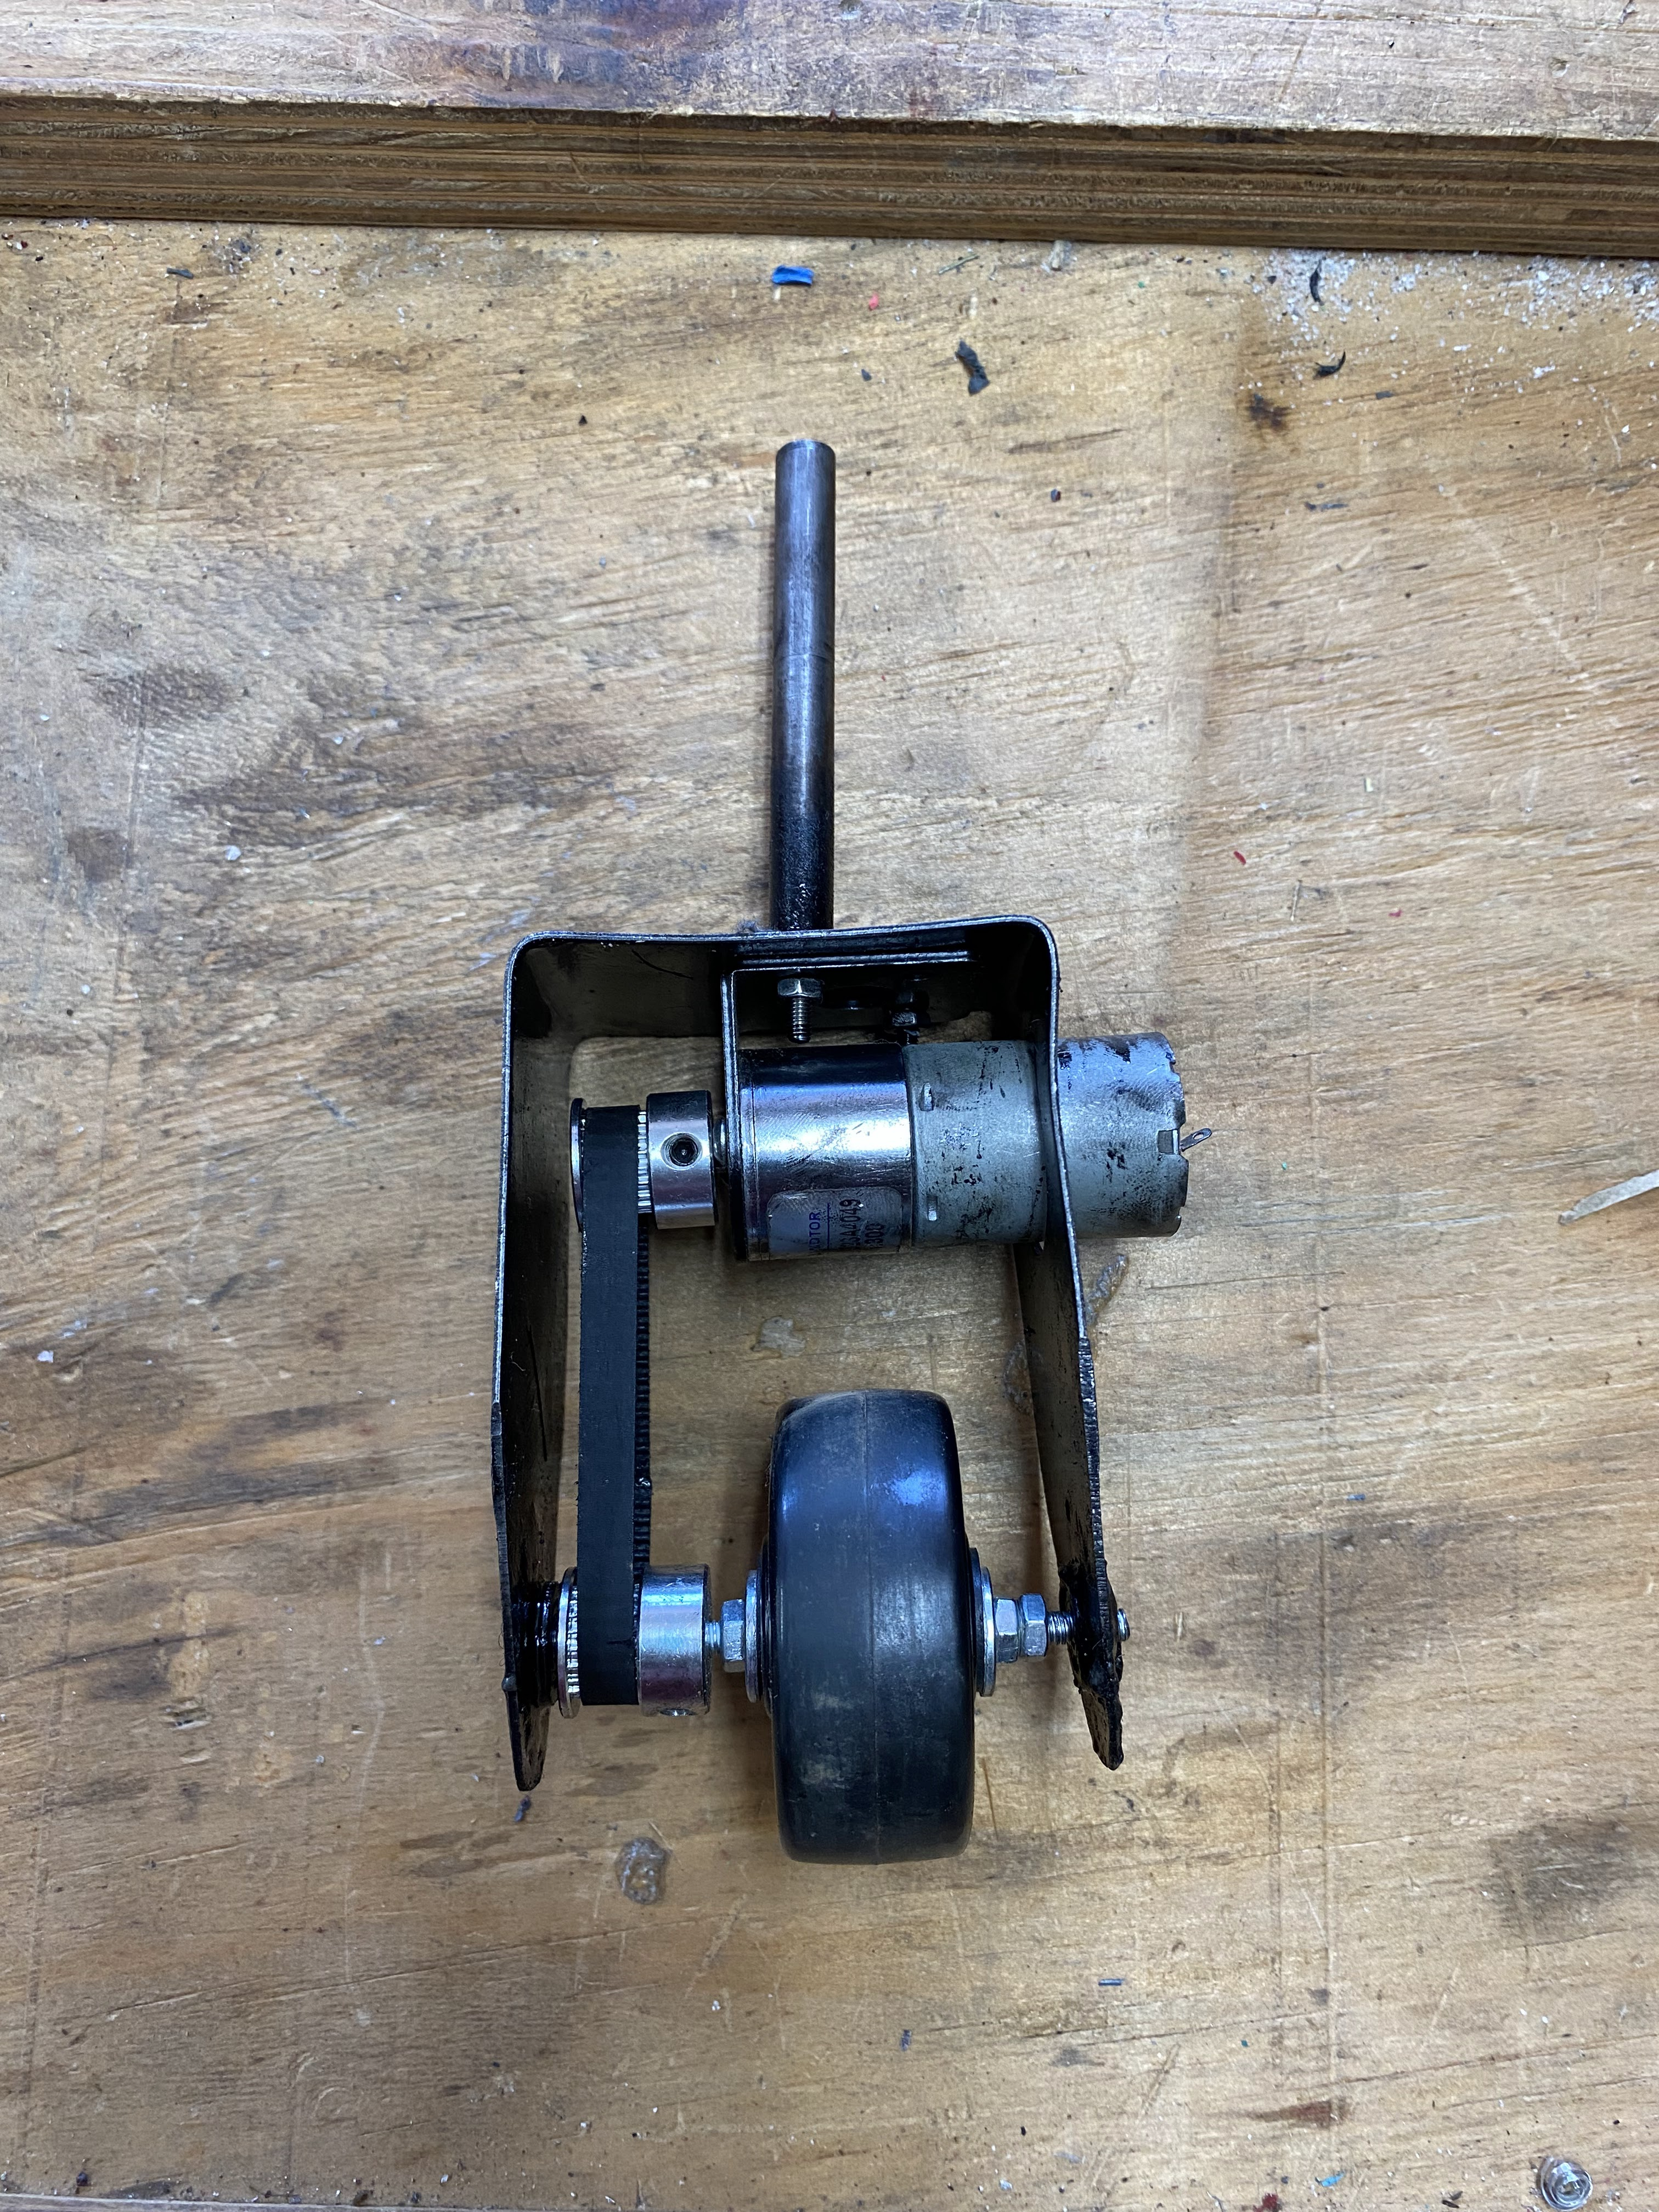
\includegraphics[scale = 0.07]{Figures/wheelFRAME1.jpg}
    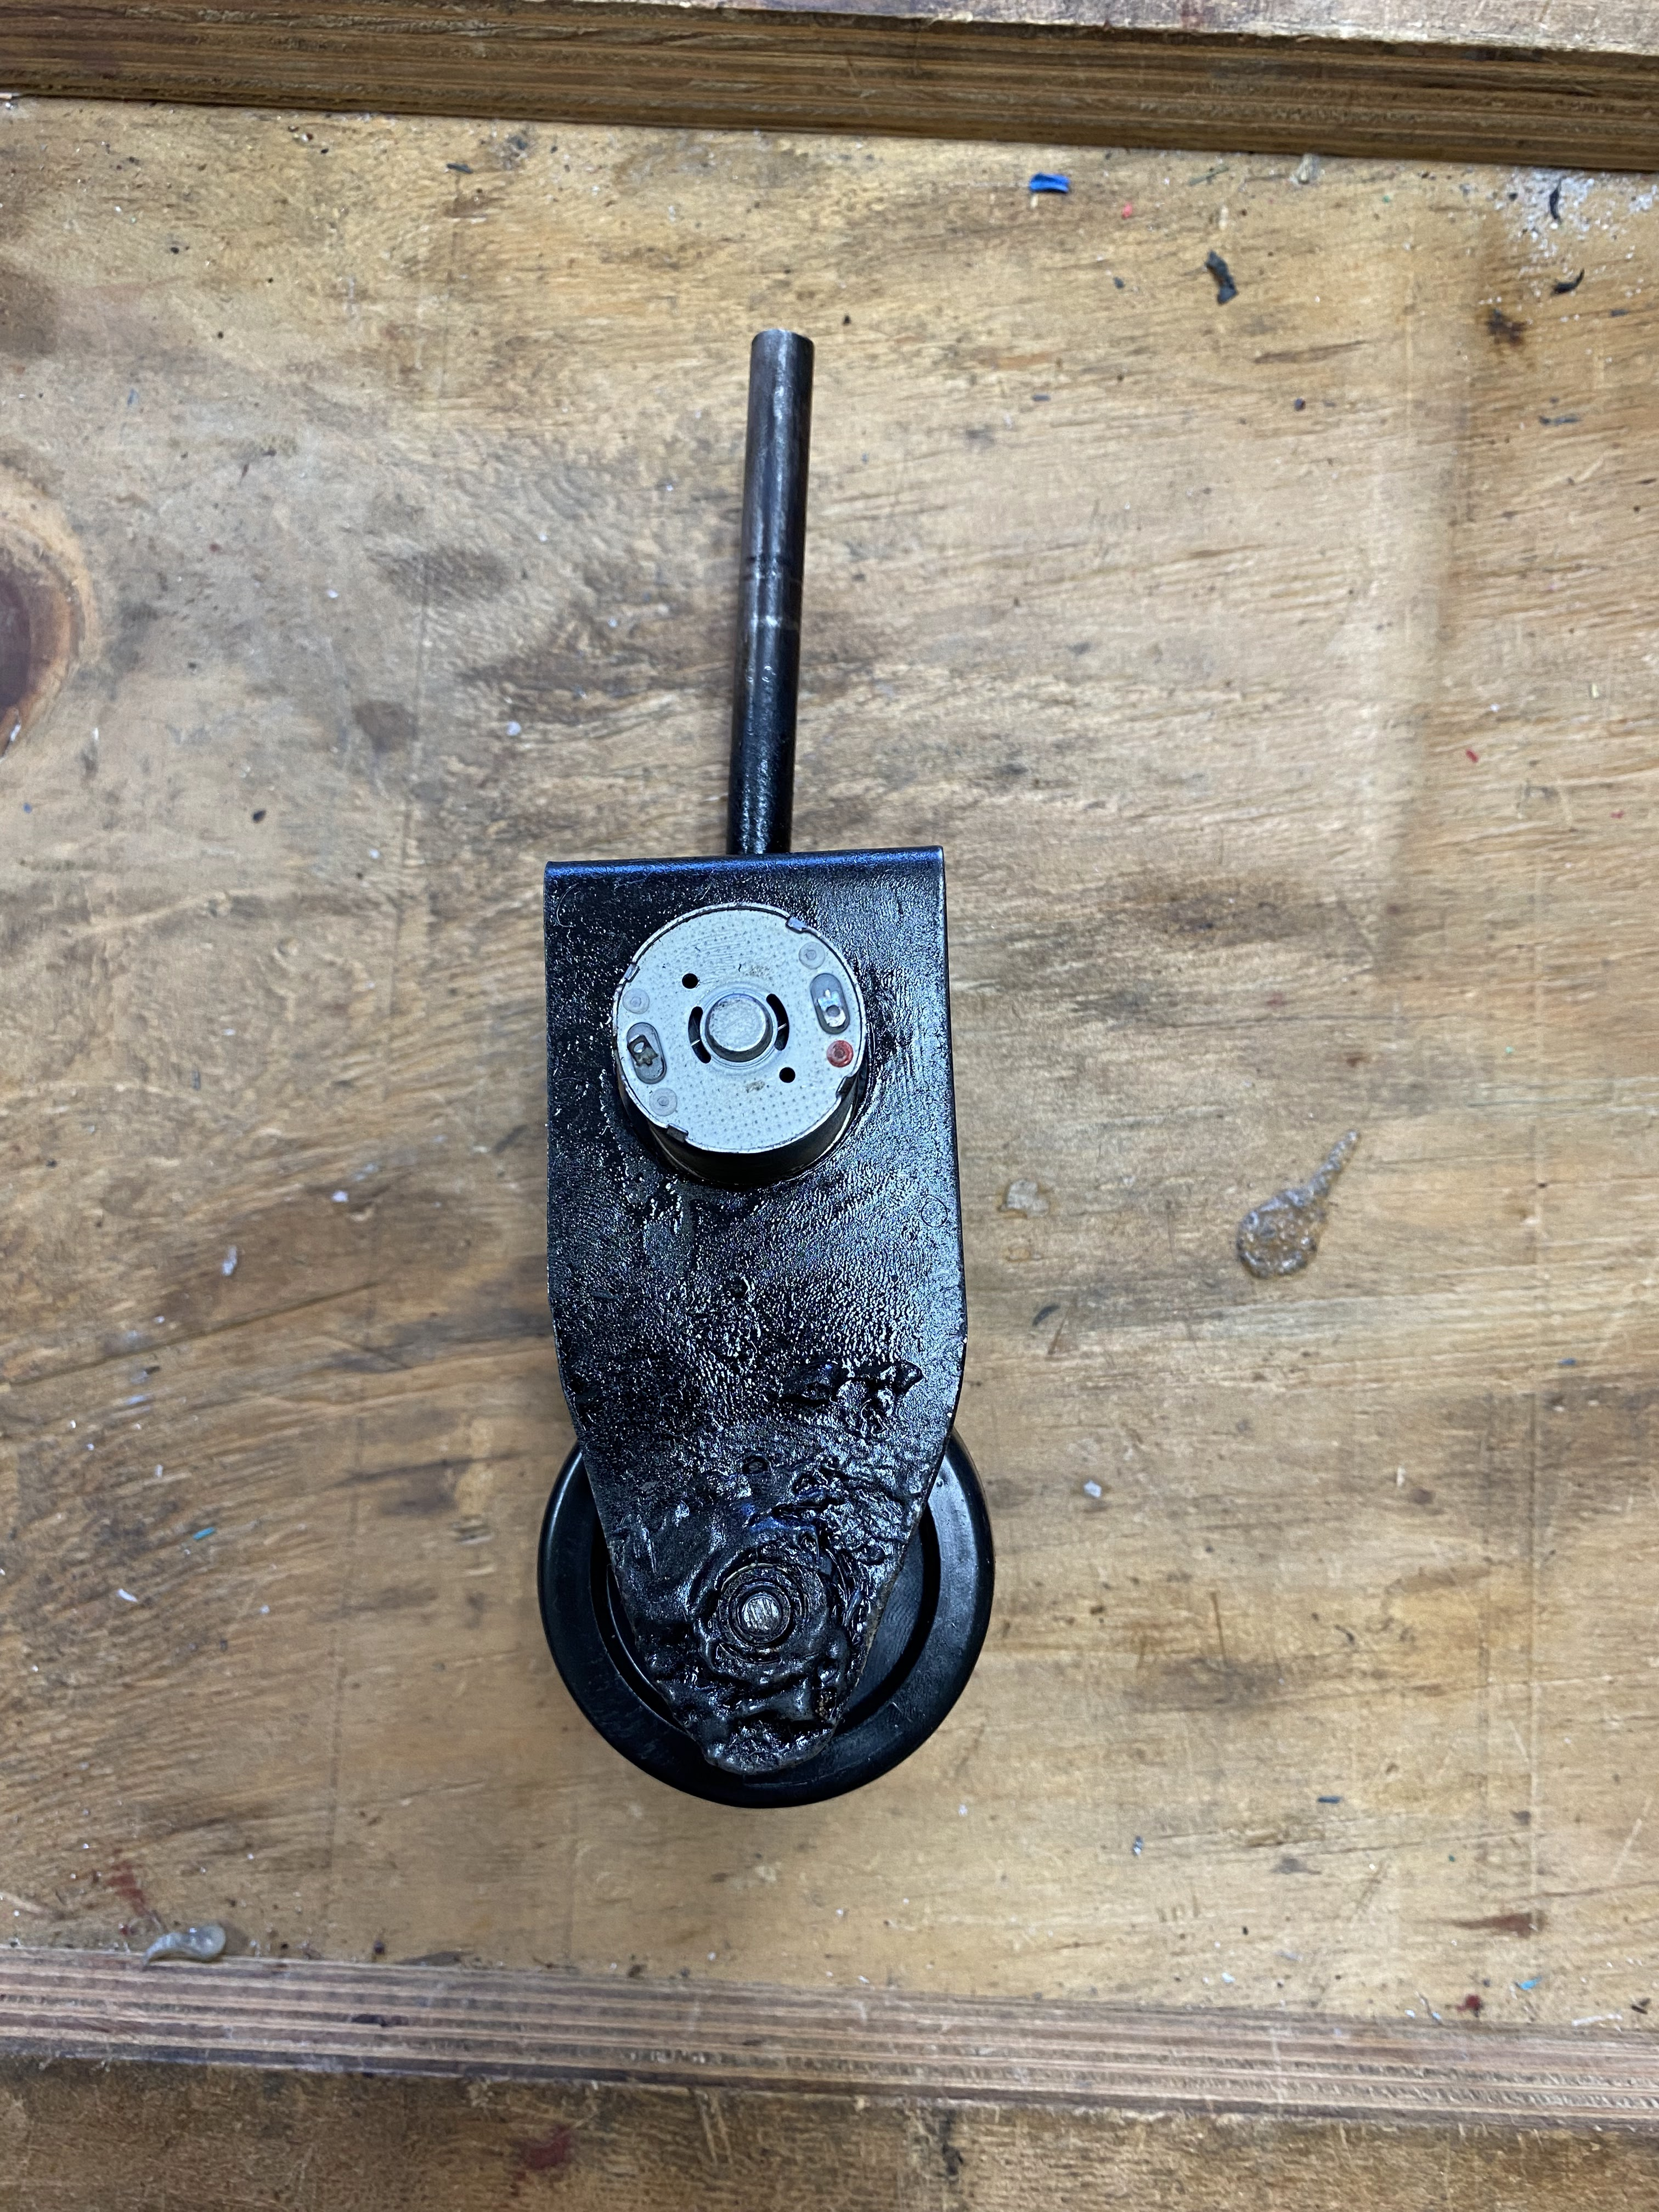
\includegraphics[scale = 0.07]{Figures/wheelFRAME2.jpg}
    \caption{Wheel-on-Frame Assembly}
    \label{fig:frameFAB}
\end{figure}

As described in Section \ref{sec:chassisFAB}, several holes were made to attach the wheel frame to the chassis. This attachment was made using an $8mm$ diameter shaft. The $8mm$ shaft would be joined to the chassis using a bearing. To join the shaft to the wheel frame, gas welding was used. Other choices considered were arc welding, Araldite adhesive, and using machine screws. These were disregarded for various reasons. Arc welding was ruled out because the heat from the electrode, which gets as high as $3500^0$ Celcius \cite{noauthor_what_nodate} would melt the sheet metal which has a melting point of $1350^0 C - 1530^0 C$.\cite{noauthor_faq_nodate}

Araldite adhesive was eliminated as there was uncertainty over whether it would hold the weight for an extended period of time. Finally, machine screws were eliminated due to the difficulty in drilling through the whole length of the $8mm$ shaft.

The final wheel-on-chassis assembly in Figure \ref{fig:wheelChassis} was done once all the individual parts were fabricated, and once the \ac{DC} motor, power transmission system and caster wheel were attached to the wheel frame.

\begin{figure}[H]
    \centering
    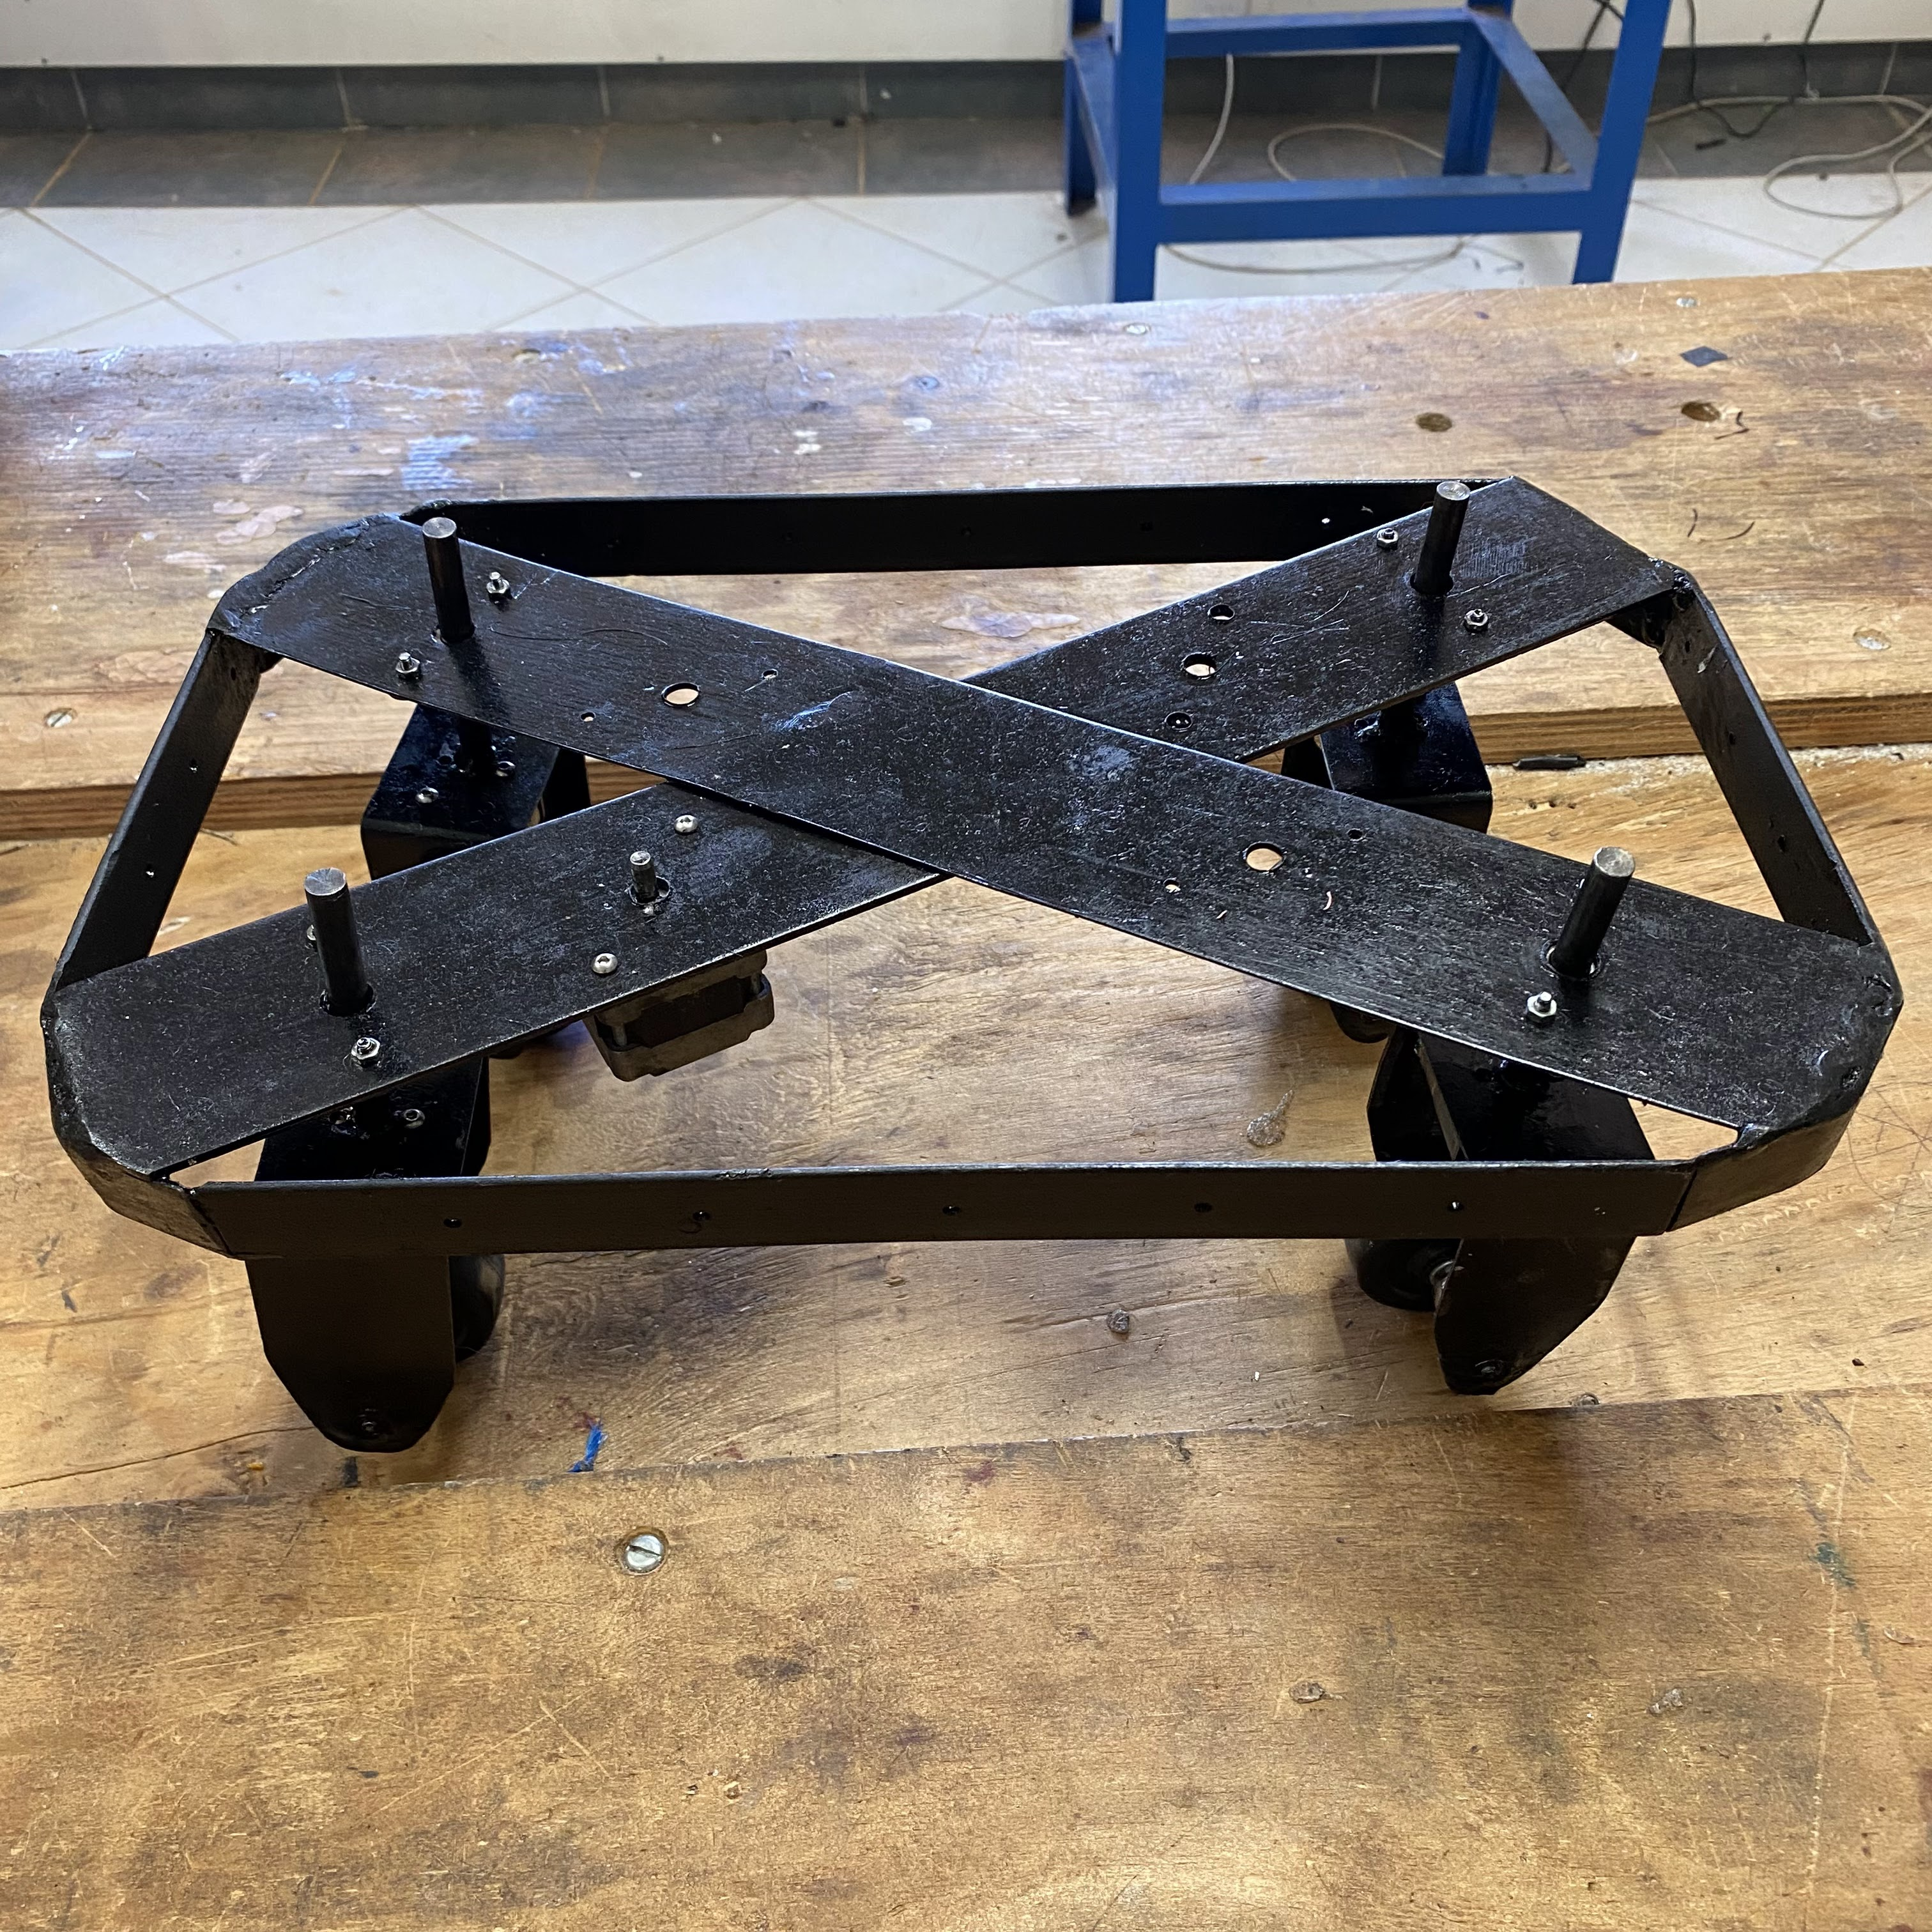
\includegraphics[scale = 0.1]{Figures/wheelCHASSISassembly.jpg}
    \caption{Wheel Frame-on-Chassis Assembly}
    \label{fig:wheelChassis}
\end{figure}



\subsection{Power Transmission}
\subsubsection{Design}
\label{sec:powerTransmission}
The main design consideration when deciding on the power transmission system was that a certain amount of power had to be transferred from the \ac{DC} motors to the caster wheels for work to be done. Several power transmission systems were considered, but ultimately belt drives were considered the best choice for the following reasons:
\begin{enumerate}[i.]
    \item There would be a centre distance between the motor and wheel shafts, a distance that would require several gears to fill which would make the design bulky. This eliminated gears as a means of transmission
    \item  The design did not require speed reduction which eliminated gear drives
    \item Belt drives require less maintenance than chain drives, for example, lubrication
    \item Belt drives are lighter than chain drives and gear drives, and given that the weight of the platform is one of the main design considerations, belt drives were the preferred choice
\end{enumerate}

Once belt drives were selected for use, other considerations were taken into account, including:
The following factors were considered when selecting a belt drive:
\begin{enumerate}[i.]
    \item The speed of the driving and driven shafts
    \item Speed reduction ratio
    \item Power to be transmitted
    \item Center distance between shafts
    \item Positive drive requirements
    \item Wheel frame dimensions
\end{enumerate}

The mobile platform was conceived as a low-speed application, with the highest speed being comparable to the speed of a walking human being. There was therefore no need for speed reduction,  meaning that the velocity ratio (speed reduction ratio) was one. This also meant that the pulleys could have the same diameter. To establish the relationship between the speed of the driving and driven shafts:

Velocity ratio:
%\ref{eq:3}:
\begin{equation}
\label{eq:3}
    \frac{N_2}{N_1} = \left(\frac{d_1}{d_2}\right)
\end{equation}

where: 
\begin{itemize}
\item \(d_1\)  is the diameter of the driver pulley
\item \(d_2\)  is the diameter of the driven pulley
\item \(N_1\)  is the speed of the driver pulley in rpm
\item \(N_2\)  is the speed of the driven pulley in rpm
\end{itemize}

Given that the velocity ratio is equal to 1, \(N_1\) = \(N_2\) and \(d_1\) = \(d_2\)

The velocity of the driving and driven shafts was determined to be equal.

From the considerations made in Section \ref{sec:wheelDesign} on the design of the wheel frame, the centre distance between the pulley attached to the \ac{DC} motor and the pulley attached to the wheel shaft was established to be $45mm$.
The diameter of the pulley was determined using bore diameter. The bore diameter is dependent on the diameter of the wheel and motor shafts. These diameters are both $5mm$ and the industry-standard outside diameter for a pulley with $5mm$ bore diameter ranges from $9.68mm$ to $37.68mm$. The industry standard is based on the common 2GT synchronous pulleys found in many small actuator applications such as 3-D printers. To make the wheel frame design more compact, a maximum pulley diameter of $16mm$ was selected for the pulley design.

\vspace{2mm}

Length of belt:

\begin{figure}[H]
    \centering
    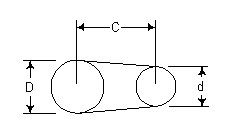
\includegraphics{Figures/NewPulley.png}
    \caption[Center distance]{Center distance\cite{noauthor_pulley_nodate}}
    \label{fig:centerdistance}
\end{figure}

\begin{equation} \label{eu_eqn}
L = \frac{\pi}{2}(d_1 + d_2) + 2C + \frac{(d_1 + d_2)^2}{4C}
\end{equation}

where: 
\begin{itemize}
\item L is the total length of the belt
\item \(d_1\)  is the diameter of the driver pulley
\item \(d_2\)  is the diameter of the driven pulley
\item C is the centre distance of the shaft
\end{itemize}

Based on the parameters established above, the total length of the belt is: 
Length of belt:
\begin{equation} \label{eu_eqn}
    \begin{aligned}
        L &= \frac{\pi}{2}(16 + 16) + 2*45 + \frac{(16 + 16)^2}{4*45}\\
        L& = 146
    \end{aligned}
\end{equation}

Arc of contact:
The angle of contact between the belt and pulleys as shown in Figure \ref{fig:centerdistance} is given by:
\begin{equation} \label{eqn4}
    \begin{aligned}
        &\theta_{\mathrm{d}}=\pi-2 \sin ^{-1} \frac{D-d}{2 C} \\
        &\theta_{\mathrm{D}}=\pi+2 \sin ^{-1} \frac{D-d}{2 C}
    \end{aligned}
\end{equation}


Since the pulleys have an equal diameter, the angle of contact of the belt on both pulleys is 90$^{\circ}$  or 1.57 radians.

Power transmitted:
Power transmitted by a belt drive:
\begin{equation}
    Power = (T_1 + T_2)v
\end{equation}

where:
\begin{itemize}
    \item \(T_1\) is the belt tension in the tight size (N)
    \item \(T_2\) is the belt tension in the slack side (N)
    v is the belt speed. Maximum drive speed is 0.5\(m/s^2\) (Section \ref{sec:initial})
\end{itemize}

Assuming that the friction is uniform throughout the arc of contact and ignoring centrifugal effects, the ratio of the tensions in the belts can be modeled by Eytlewein’s formula:
\begin{equation}
    \frac{T_1}{T_2} = e^{\mu \theta}
\end{equation}

where:
\begin{itemize}
    \item \(\theta\) is the angle of contact
    \item \(\mu\) is the coefficient of friction
\end{itemize}

The maximum allowable tension, \(T_{1,max}\), on the tight side of a belt, depends on the allowable stress, \(\alpha_{max}\), of the belt material in this case rubber. 
\begin{equation}
    T_{1, max} = \alpha_{max}A
\end{equation}

where:
\begin{itemize}
    \item A is the cross-sectional area of the belt, i.e., \begin{equation}
        A = bt
    \end{equation}
    \item b is the belt width
    \item t is the belt thickness
\end{itemize}

For standard 2GT synchronous pulleys, the maximum tooth width is 11mm and maximum thickness is 1.8mm.
The maximum allowable stress for rubber is 5MPa.
\par
Therefore:
\begin{equation}
    \begin{aligned}
         T_{1,max}& =5*10^6*\frac{11}{1000}*\frac{1.8}{1000}\\
         & = 99N
    \end{aligned}
\end{equation}
Given that:

\begin{equation}
    \begin{aligned}
       \frac{T_1}{T_2}&= e^{\mu\theta},
        and\  
        T_1 = 99N,   \mu =0.32,  \theta= 1.57 radians\\
        T_2 &= 61.81N
    \end{aligned}
\end{equation}

Power transmitted by the belt drive:
\begin{equation}
    \begin{aligned}
        P &= (T_1 + T_2)v \\
        P &= (T_1 + T_2)*0.5\\
        P &= 80.4W
    \end{aligned}
\end{equation}
Torque transmitted by the belt drive:
\begin{equation}
    \begin{aligned}
        T &= (T_1 + T_2)r\\
        T &= (T_1 + T_2)\frac{8}{1000}\\
        T &= 1.28Nm
    \end{aligned}
\end{equation}

This torque value is important when considering the kind of \ac{DC} motor to use. 

\subsubsection{Fabrication}
Based on design considerations, the pulley was selected from the industry standard 2GT synchronous pulleys. These pulleys have a bore diameter of $6mm$ and a smaller shaft can be screwed tight using an Allen key. The pulley has twenty teeth along its diameter, along which the belt fits perfectly as in Figure \ref{fig:beltPulley}.

\begin{figure}[H]
    \centering
    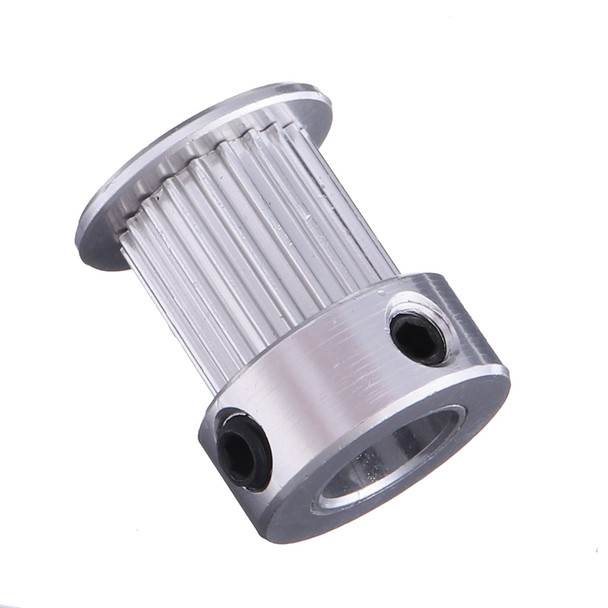
\includegraphics[scale = 0.35]{Figures/2gtPulley.jpg}
    \caption{Pulley Selected}
    \label{fig:newPulley}
\end{figure}

The belt also exists in standard form as represented in Figure \ref{fig:timingBelt}. 
\begin{figure}[H]
    \centering
    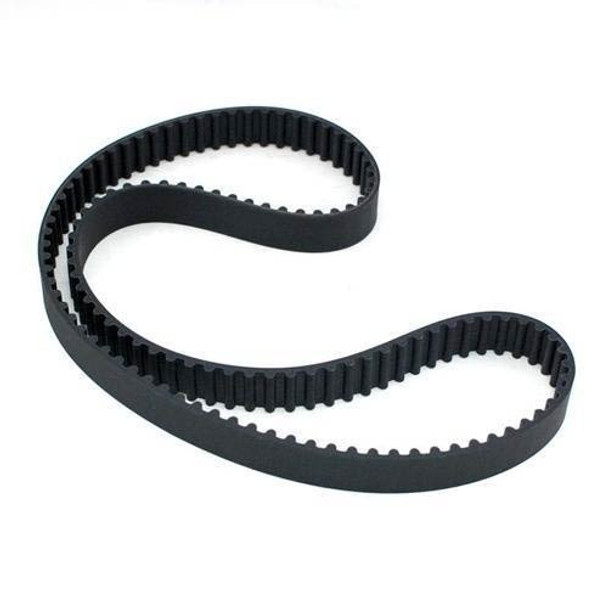
\includegraphics[scale = 0.35]{Figures/timingBelt.jpg}
    \caption{Timing Belt Selected}
    \label{fig:timingBelt}
\end{figure}

\begin{figure}[H]
    \centering
    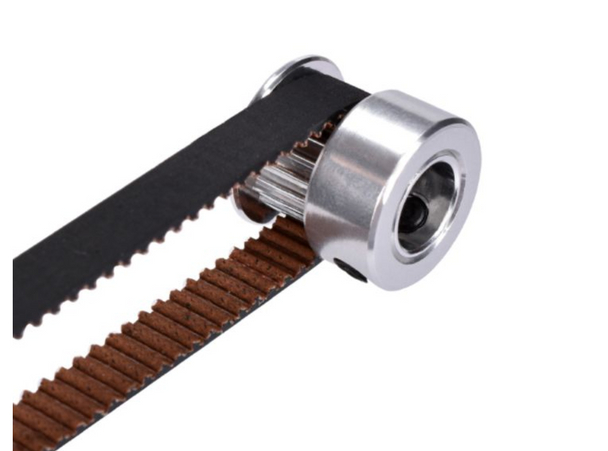
\includegraphics[scale = 0.4]{Figures/beltPulley.jpg}
    \caption{Timing Belt and Pulley}
    \label{fig:beltPulley}
\end{figure}

\subsection{Bearing Selection}
\subsubsection{Design}
The choice of bearing depended on the type of payload the platform was going to carry. This would dictate whether the load was axial or radial, or a combination of the two. A very large axial load would require the use of axial or thrust bearings which withstand force in the same direction as the shaft. Roller and radial ball bearings, on the other hand, are designed to withstand radial loads. However, some radial ball bearings are able to withstand both medium-large radial and axial loads \cite{noauthor_4_nodate}, which makes them a perfect fit for the platform. Moreover, radial ball bearings are easy to acquire due to their affordability. 
The bore diameter of the bearings was dependent on the diameter of the shafts. The wheel shaft diameter was listed as being $1mm$ whereas the wheel frame shaft had a diameter of $8mm$. Bearings with these respective diameters were chosen for the design.

\subsubsection{Fabrication}
When it came to attaching the bearing to the chassis in Figure \ref{fig:chassisFAB}, a bearing housing had to be machined. However, to save time and resources, a bearing with a fitted housing and attachment block was purchased. It was a much cheaper option and turned out to be very effective. 

\begin{figure}[H]
    \centering
    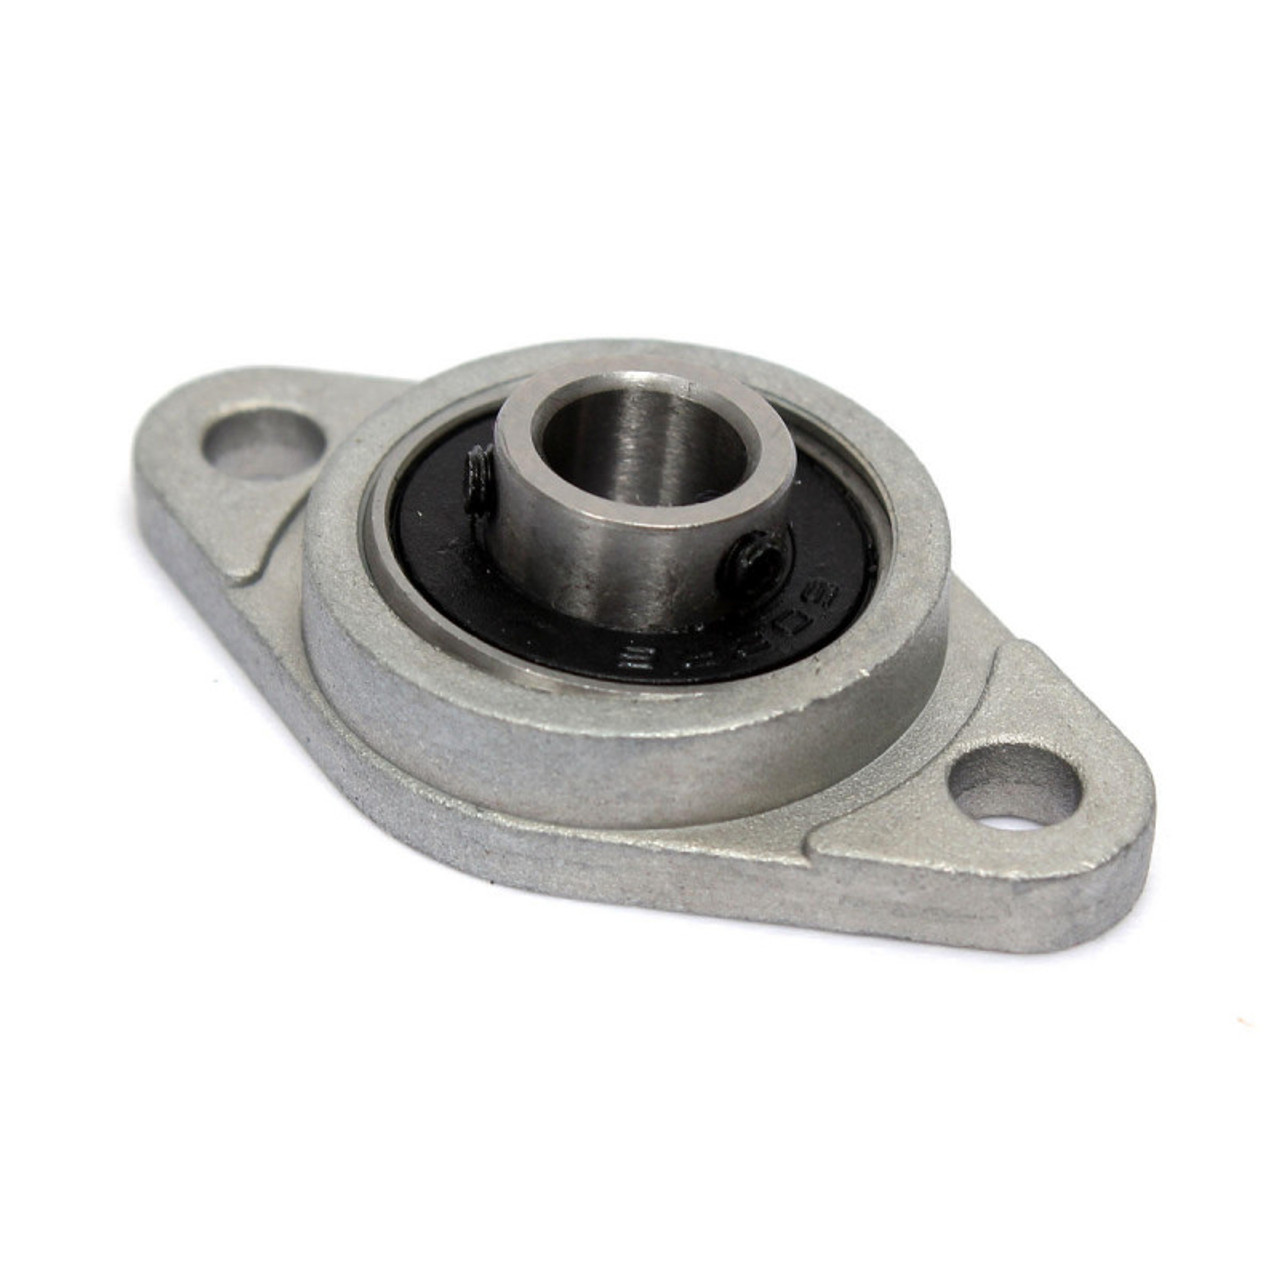
\includegraphics[scale = 0.2]{Figures/pillowBlock.jpg}
    \caption{$8mm$ Bearing with Housing}
    \label{fig:pillowBlock}
\end{figure}
The bearing in Figure \ref{fig:pillowBlock} also had a provision for fitting shafts with a diameter less than $8mm$ with screws that could be tightened with an Allen key.

\begin{figure}[H]
    \centering
    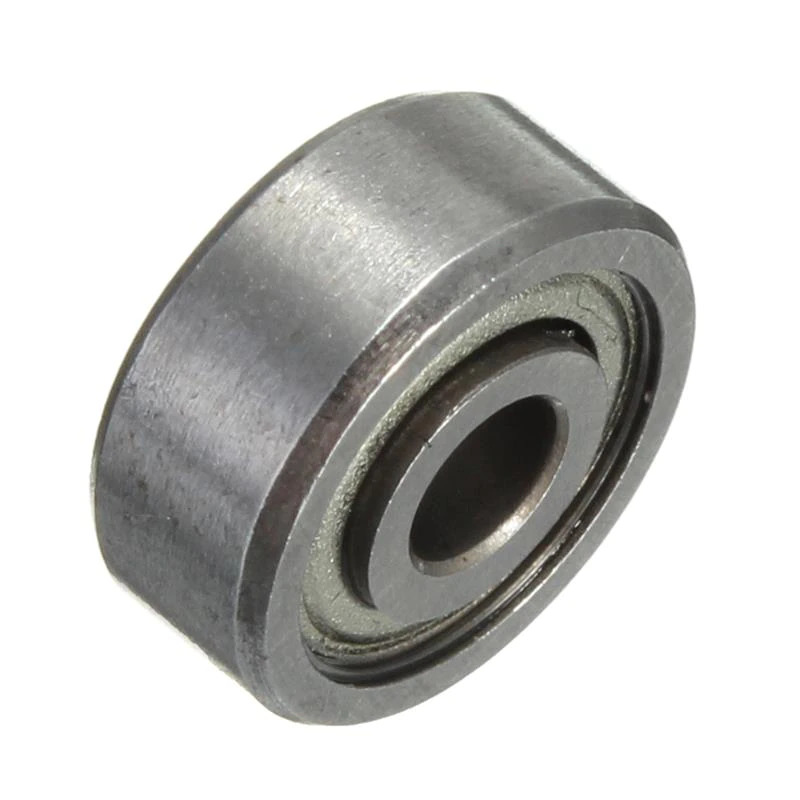
\includegraphics[scale = 0.25]{Figures/wheelBearing.jpg}
    \caption{$1mm$ Bearing}
    \label{fig:wheelBearing}
\end{figure}

\subsection{Motor Selection}
\label{sec:motor}
\subsubsection{Design}
The motor is responsible for supplying the drive to the transmission system responsible for the movement of the robot. There are numerous motor types that can be used in robotic applications. Each type of motor serves a distinct purpose. The motors help the robot move and act as actuators in the mechanical design of the robot. Since this is a mobile robot with a small payload size, \ac{AC} motors are ruled out. The remaining \ac{DC} motors used for locomotion are:
\begin{enumerate}[i.]
    \item Brushed \ac{DC} motors use brushes to conduct current between the source and the armature. There are several types of brushed \ac{DC} motors, but permanent magnet \ac{DC} motors are used in robotics. These motors have a high torque-to-inertia ratio. Brush \ac{DC} motors are capable of producing torque three to four times greater than their rated torque. The brush \ac{DC} motors have two terminals. When a voltage is applied across the two terminals, a proportional speed is output to the brush \ac{DC} motor's shaft.

    \item Brushless \ac{DC} motors are built similarly to brushed \ac{DC} motors, but they are controlled by closed-loop controllers and require inverters or \ac{SMPS} for power. Permanent magnets rotate a fixed armature in these motors. Unlike Brush \ac{DC} motors, they have a closed-loop electronic controller instead of a commutator assembly. These motors are typically used in industrial robotics where precise motion and positioning control are required. These motors, however, are quite expensive and involve complex construction and electronics.

    \item Geared \ac{DC} motors are a more advanced version of brush \ac{DC} motors. A gear assembly is attached to the motor. The motor's speed is reduced as the torque increases thanks to the gear assembly. The speed of the \ac{DC} motor can be reduced while increasing torque by using the proper combination of gears to the motor. This ensures that the motor rotates steadily and that it can be stopped or changed speed in a controlled manner. \ac{DC} motors operate within a specific voltage range, and the higher the input voltage, the higher the \ac{RPM}.
\end{enumerate}

When selecting the right motor to use in this application the following design considerations were made:
\begin{enumerate}
    \item a high torque motor of approximately $1 Nm$ that could carry a payload of $20 kg$ (Section \ref{sec:initial}) at low speed
    \item the operating voltage, which has a direct correlation with the power drawn from the battery, thus influencing the capacity of the battery
    \item Cost and availability
\end{enumerate}  
From the motor choices listed above, the geared \ac{DC} motor was selected for this application. This choice was influenced by various parameters showcased in Table \ref{table:comparedifferentmotrs}.

\begin{table}[ht]
  \begin{center}
    \leavevmode
    \hangcaption[Comparison between different motors]{Comparison between different motors}
    \begin{tabular}{|c|c|c|c|}\hline
    Parameters & Brushed \ac{DC} motors & Brushless \ac{DC} motors & Geared \ac{DC} motors \\\hline
    Speed & Fast & High & Low \\\hline
    Torque & Low & Low & High \\\hline
    Cost & Inexpensive & Expensive & Inexpensive \\\hline
    Availability & Available & Available & Available \\\hline
    Operating Voltage & $6 V$ - $12 V$ & $12 V$ & $6 V$ - $12 V$ \\\hline
    Lifetime & Short & Long & Short \\\hline
    Efficiency & Low & High & Low \\\hline
    Noise & High & Low & Low \\\hline
    \end{tabular}
    \label{table:comparedifferentmotrs}
  \end{center}
\end{table}

Once the geared \ac{DC} motor was chosen, the specific properties of the right geared \ac{DC} motor had to be established. The following considerations were taken when selecting this motor.

\begin{enumerate}[i.]
    \item  Nominal Voltage. The higher the voltage, the less current will be needed to supply the electrical power to the motors. A $6 V$ motor will draw twice as much current as a $12 V$ motor for the same application 
    \item No Load \ac{RPM} and full load \ac{RPM}
    \item Stall current and Stall torque - The system ought to be designed to never allow the motor to come anywhere near this point, This can be done by ensuring the motor operated at least 30\% of the stall torque.
    \item Gear down - This helps to achieve the required torque at the output of the shaft and allows the transmission unit to run at a gear ratio of 1:1. The output speed is reduced to a manageable level while the torque is increased.
    \item Rotary encoders. This would be a great addition, but finding a geared \ac{DC} motor with the rotary encoder attached to it is difficult.
\end{enumerate}

Torque is another important element when selecting the right motor. This torque, therefore, has to be determined as follows:
\begin{figure}[h]
    \centering
    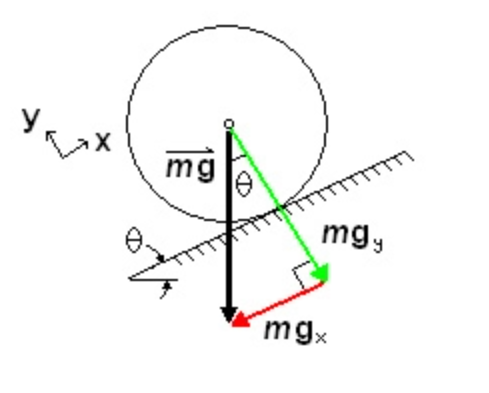
\includegraphics[scale=0.5]{Figures/simpleTorque.png}
    \caption{Simple Torque Representation On an Inclined Surface}
    \label{fig:simpletorque}
\end{figure}

From Figure \ref{fig:simpletorque} with a $5^{\circ}$ inclined surface, only one component of its weight, $mg_x$ parallel to the surface, causes the robot to move downwards. The other component, $mg_y$, is balanced by the normal force the surface exerts on the wheels. $mg_x$ is calculated as shown by Equation \ref{mgxcalculations} and $mg_y$ is calculated as shown by Equation \ref{mgycalculations}


\begin{equation} \label{mgxcalculations}
\begin{split}
mg_x & = mg * sin (\theta) \\
& = 45 * 9.81 * sin (5) \\
& = 38.4749 N 
\end{split}
\end{equation}

\begin{equation} \label{mgycalculations}
\begin{split}
mg_y & = mg * cos (\theta) \\
& = 45 * 9.81 * cos (5) \\
& = 439.7701 N
\end{split}
\end{equation}


For the robot not to slide down the incline, there must be friction between the wheel and the surface. 
The torque (T) required is given by equation \ref{torqueeqn}.

\begin{equation} \label{torqueeqn}
T = f * R
\end{equation}

To select the proper motor, we must consider the worst-case scenario, where the robot is not only on an incline but accelerating up it.
Note now that all forces ($F$) are along the x and y axes. The forces in the x-direction are balanced as shown in equation \ref{balanceforces}

\begin{equation} \label{balanceforces}
\begin{split}
F_x & = m * a  \\
& = f - m g_x \\
& = \frac{T}{R} - m g_x
\end{split}
\end{equation}

% \begin{flushleft} \label{balanceforces}

% \end{flushleft}

\begin{equation} \label{totaltorqueeqn}
T = R * M *( a + g * sin(\theta))
\end{equation}

This torque given by equation \ref{totaltorqueeqn} value represents the total torque required to accelerate the robot up an incline. However, this value must be divided by the total number ($N$) of drive wheels to obtain the torque needed for each drive motor. The final point to consider is the efficiency ($e$) of the motor, gearing, and wheel (slip). This results to the torque required by each wheel as shown by equation \ref{totaltorqueeqnwithefficiency}

\begin{equation} \label{totaltorqueeqnwithefficiency}
T = \frac{100}{e} * \frac{R * M *( a + g * sin(\theta))}{N}
\end{equation}

The value for efficiency here represents the total efficiency, as shown by equation \ref{totalefficiency}, of the system and can be estimated as follows:
\begin{itemize}
    \item Battery to Motor Controller: 90\% efficient
    \item Motor Controller to Motors: 70\% efficient
    \item Transmission to Wheels 80\% efficient
\end{itemize}
The lost energy is transferred mostly to heat and noise.

\begin{equation} \label{totalefficiency}
\begin{split}
e & = 0.9 * 0.7 * 0.8 \\
& = 50.4\% \\
\end{split}
\end{equation}

With a total efficiency of the system as $50.4\%$ torque required by each wheel is calculated as shown in equation \ref{totaltorque}.

\begin{equation} \label{totaltorque}
\begin{split}
T & = \frac{100}{50.4} * \frac{0.015 * 45  *( 0.25 + 9.81 * sin(5))}{4} \\
& = 0.37 Nm \\
\end{split}
\end{equation}

With this a motor of $12V$ $250$ \ac{RPM} \ac{DC} motor of $0.8629 N/m$ in torque can suffice for this operation. This motor can provide the required torque for this application but the Speed will be reduced to $0.3927 m/s$ as shown by equation \ref{speedmpers} which is not far off from the expected $0.5 m/s$.

\begin{equation} \label{speedRadians}
w = \frac{2 * \pi * N}{60}
\end{equation}

\begin{equation} \label{speedmpers}
\begin{split}
v & = r * w\\
& = 0.015 * \frac{2 * \pi * 250}{60} \\
& = 0.3927 m/s 
\end{split}
\end{equation}

The total power ($P$) per motor can be calculated using the following relation:


\begin{equation} \label{totalefficiency}
\begin{split}
P & = T * w\\
& = 0.37 * \frac{2 * \pi * 250}{60} \\
& = 9.6866W 
\end{split}
\end{equation}

\begin{equation} \label{totalefficiency}
\begin{split}
I & = \frac{P}{V}\\
& = \frac{9.6866 W}{12 V} \\
& = 0.8072 A
\end{split}
\end{equation}


The maximum current that id drawn from a battery is $0.4843A$ to be supplied to the motors.

Finally, the capacity ($C$) of the battery pack required can be estimated using the equation \ref{batterycap}:

\begin{equation} \label{batterycap}
\begin{split}
C & = I * t\\
& = 0.8072 * 1 \\
& = 0.8072Ah \\
& = 0.8072 * 8 \\ 
& = 3.2288 Ah \\
\end{split}
\end{equation}

With a $3.2 Ah$ battery the motors will be able to run the mobile platform for 1hr without recharging.

\subsubsection{Implementation}
Having calculated the torque required from the \ac{DC} motor in Section \ref{sec:motor}, a geared \ac{DC} motor that met all the specified conditions was chosen. The particular motor, shown  in Figure \ref{fig:dcMotor} is a 12V, 300rpm and 0.8629Nm motor that has enough torque to move a $20kg$ payload. The motor also coincides with the dimensions listed when designing for the wheel frame in section \ref{sec:wheelDesign} as it has a diameter of $25mm$ and a total length of $50mm$

\begin{figure}[H]
    \centering
    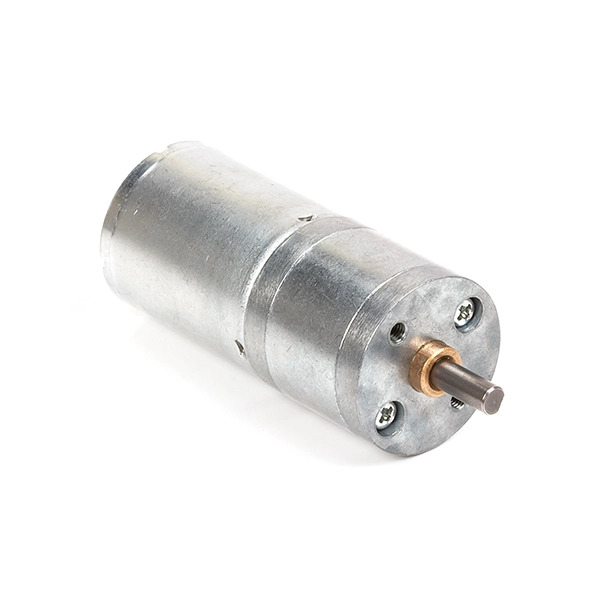
\includegraphics[scale = 0.4]{Figures/dcMotor.jpg}
    \caption{Geared \ac{DC} Motor}
    \label{fig:dcMotor}
\end{figure}

This motor torque is also less than the torque determined for the power transmission system in section \ref{sec:powerTransmission}. This means that the belt drives considered can transmit the power from the \ac{DC} motor.

\subsubsection{Design Changes}
The original plan was to apply geared \ac{DC} motors for both drive and steering functions. However, a realisation was made that \ac{DC} motors would not provide feedback data on the exact position of the shaft, information that was crucial in controlling the direction of the platform. For this purpose, an encoded \ac{DC} motor or a standard stepper motor were the ideal choices. However, the encoded \ac{DC} motor was difficult to acquire locally, mostly due to empty stores or blatant overpriced quotations. On the other hand, stepper motors were easy to acquire, even from second-hand shops, a choice that proved financially sound.
\par
A stepper motor of the same specifications as the \ac{DC} motor selected in Section \ref{sec:motor} was purchased for direction control. This meant there was a total of four geared \ac{DC} motors for drive, and at least two stepper motors for direction control.
\par
Having changed to a different motor altogether, there was concern that the motor driver modules selected for the platform in Section \ref{sec:motorControl} would be unable to control the stepper motor. However, this was not the case because the drivers could each support one stepper motor meaning that the motor control design did not have to change.

\begin{figure}[H]
    \centering
    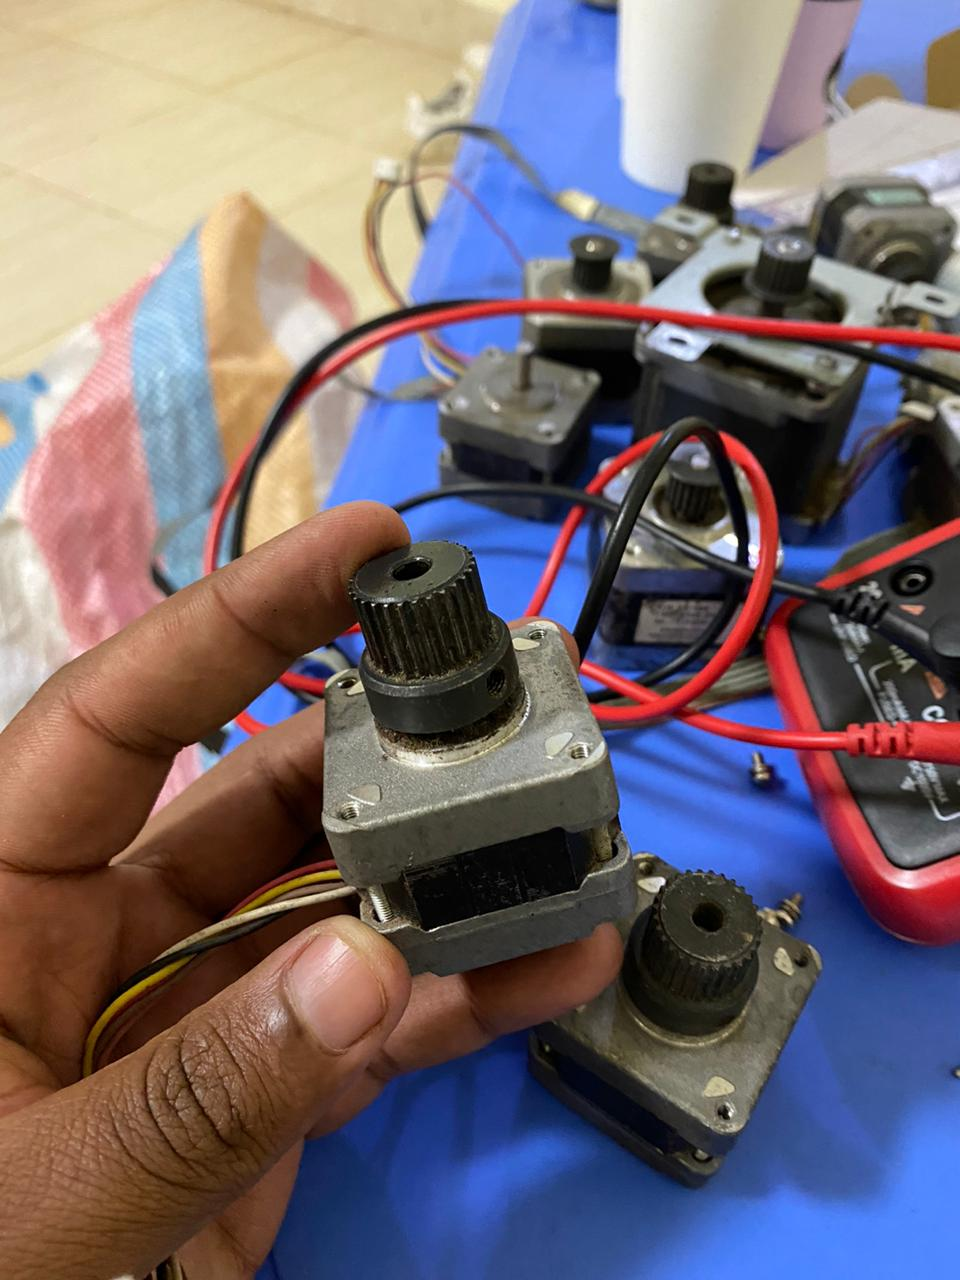
\includegraphics[scale = 0.3]{Figures/stepperMotor.jpg}
    \caption{Stepper Motor Selected}
    \label{fig:stepperMotor}
\end{figure}

\subsection{Motor Control}
\label{sec:motorControl}
\subsubsection{Design}
Motor control is achieved using a motor driver module. Motor direction control is achieved using an H-bridge circuit whereas speed control is achieved using \ac{PWM}
Some of the design considerations that were made when choosing a motor driver were: 

\begin{enumerate}[i.]
    \item Ability to both control speed and rotations
    \item The higher the number of motor outputs the better
    \item The operating voltage should be inclusive of our motor voltage of 12V.
    \item The higher the efficiency the better. \ac{MOSFET} controlled drivers have a higher efficiency that \ac{BJT}.
    \item A small form factor would be better
    \item Maximum current it can supply to the motors should be approximately 1A needed to generate our required torque of $0.37 N m$
\end{enumerate}

Several motor drivers were considered, including the L293D circuit. However, The Satima S2 motor driver, a custom driver based on DRV880 that can be used to drive either 2 bidirectional or 4 unidirectional DC motors, was best suited for this application. This is because it can operate a 12V motor voltage, can supply up to a maximum of 3A per channel and High-Noise-Immunity Inputs. Furthermore, it is \ac{MOSFET} controlled making it have higher efficiency compared to the \ac{BJT}-powered L293D.

\begin{figure}[H]
    \centering
    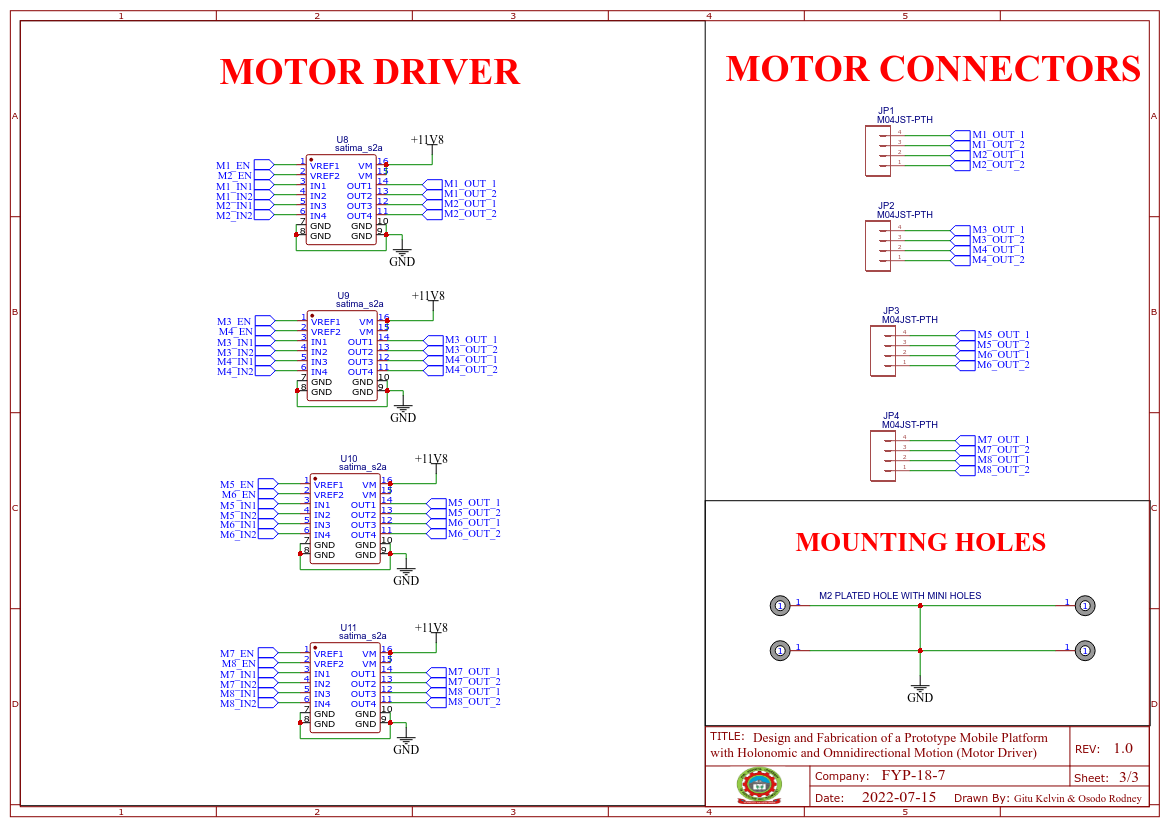
\includegraphics[scale = 0.4]{Figures/MPmotorDriver.png}
    \caption{Motor Driver Schematic}
    \label{fig:motordriverschematic}
\end{figure}

Figure \ref{fig:motordriverschematic} shows the Motor Driver schematic, which is a part of the Mobile Platform. There are 8 motors controlled by 4 motor drivers which can be able to control 2 motors per motor driver. The Connectors are JST connectors as they are strong and reliable. The mounting holes are connected to the ground as they will be screwed on to the platform. The schematic was designed using the open-end software EasyEDA.
\par
Once the schematics were designed, the actual \ac{PCB} in Figure \ref{fig:mobileplatformmain} that would host the circuit for motor control was also designed and simulated. The same software, EasyEDA was used for this function.

\subsubsection{Fabrication}
The satima motor driver in Figure \ref{fig:satimaDriver} and the \ac{PCB} in Figure \ref{fig:PCB} were manufactured based on their individual scematics. The choice was made to use \ac{PCB} companies such as Gearbox or JLPCB as the components would require complex fabrication techniques that could not be achieved manually. For this case, JLPCB was the manufacturer of choice. All that had to be done was send the relevant Gerber files generated from the design processs to the manufacturer and pay for the service. A Gerber file is an open ASCII vector format file that contains information on each physical board layer of your \ac{PCB} design \cite{team_gerber_2019}. Circuit board objects, like copper traces, vias, pads, solder mask and silkscreen images, are all represented by a flash or draw code, and defined by a series of vector coordinates. These files are used by \ac{PCB} manufacturers to translate the details of your design into the physical properties of the PCB. The Gerber files are generated by the \ac{PCB} design software, in this case, EasyEDA.
\begin{figure}[H]
    \centering
    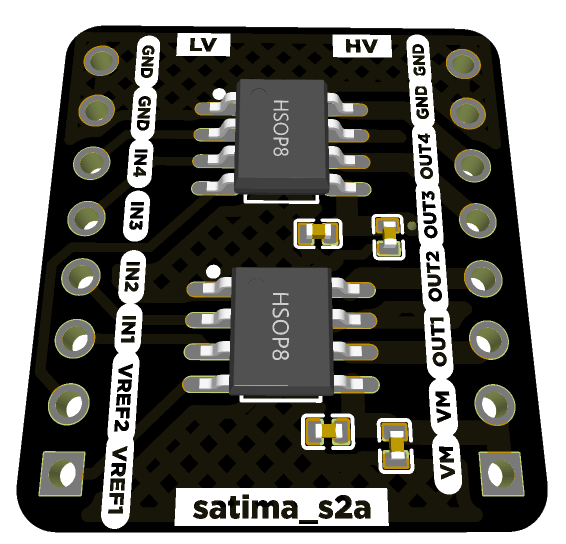
\includegraphics[scale = 0.4]{Figures/satimaDriver.png}
    \caption{Satima Motor Driver}
    \label{fig:satimaDriver}
\end{figure}


\subsection{Platform Control Electronics}
\label{sec:platformControl}

This represents the brain of the mobile platform and is responsible for converting user input to motor rotation and translational values. The main compute platform is responsible for controlling the motors individually to achieve holonomic control.
The main components of the platform control are: the main microcontroller, power supply, and the Wi-Fi client. The schematic designs in Figure \ref{fig:mobileplatformmain} were developed using EasyEDA software.

\begin{figure}[H]
    \centering
    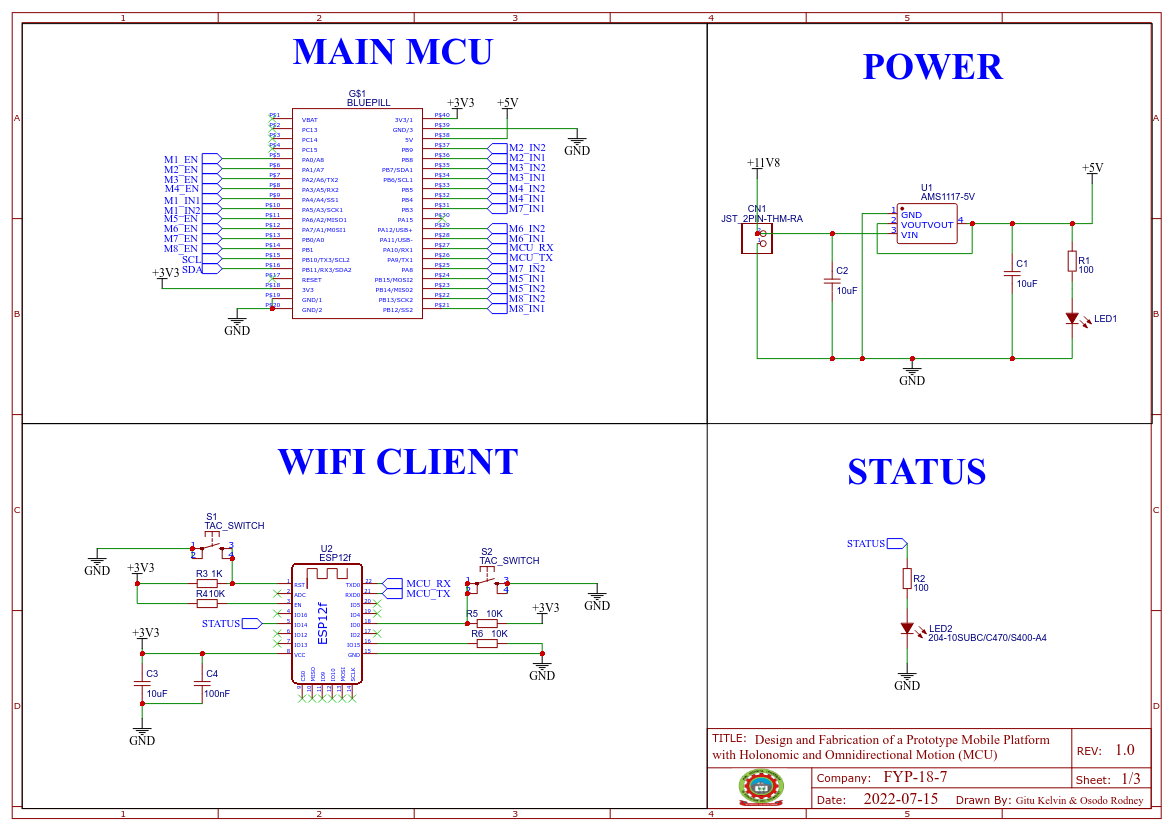
\includegraphics[scale=0.4]{Figures/MPmain.png}
    \caption{Mobile Platform Main Schematic View}
    \label{fig:mobileplatformmain}
\end{figure}


The considerations that went into selecting the microcontroller were:
\begin{enumerate}[i]
    \item It should be compatible with all auxilliary components including the motor and the inertial measuring sensor
    \item It should have on board features such as integrated Wi-Fi support and USB port
    \item It should have enough processing power to reduce latency during operations such as wireless communication.
    \item Its memory should be enough to accommodate the written program with all of its functionality.
    \item It should have the desired number of GPIO pins.
\end{enumerate} 

\par
The STM32 and Arduino microcontrollers were considered as they are the most common and prevalent in the market. The STM32 microcontroller, more specifically STM32F103C8T6 was chosen as main \ac{MCU}, and the main deciding factor was the number of pins on the \ac{MCU}. It has 40 pins which would comfortably accommodate the more than 24 pins required to operate eight \ac{DC} motors.
\par
For the Wi-Fi client, the ESP-12f was chosen. This module supports the standard IEEE802.11 b/g/n protocol, a complete
TCP/IP protocol stack. It adds networking capabilities to existing devices and can be used to build separate network controllers. It is also highly cost effective compared to other modules such as ESP32.


The motor driver schematics in Figure \ref{fig:motordriverschematic} and the platform control schematics in Figure \ref{fig:mobileplatformmain} were incorporated into one circuit and used to generate the main \ac{PCB} in Figure \ref{fig:mobileplatformmain}.

\begin{figure}[H]
    \centering
    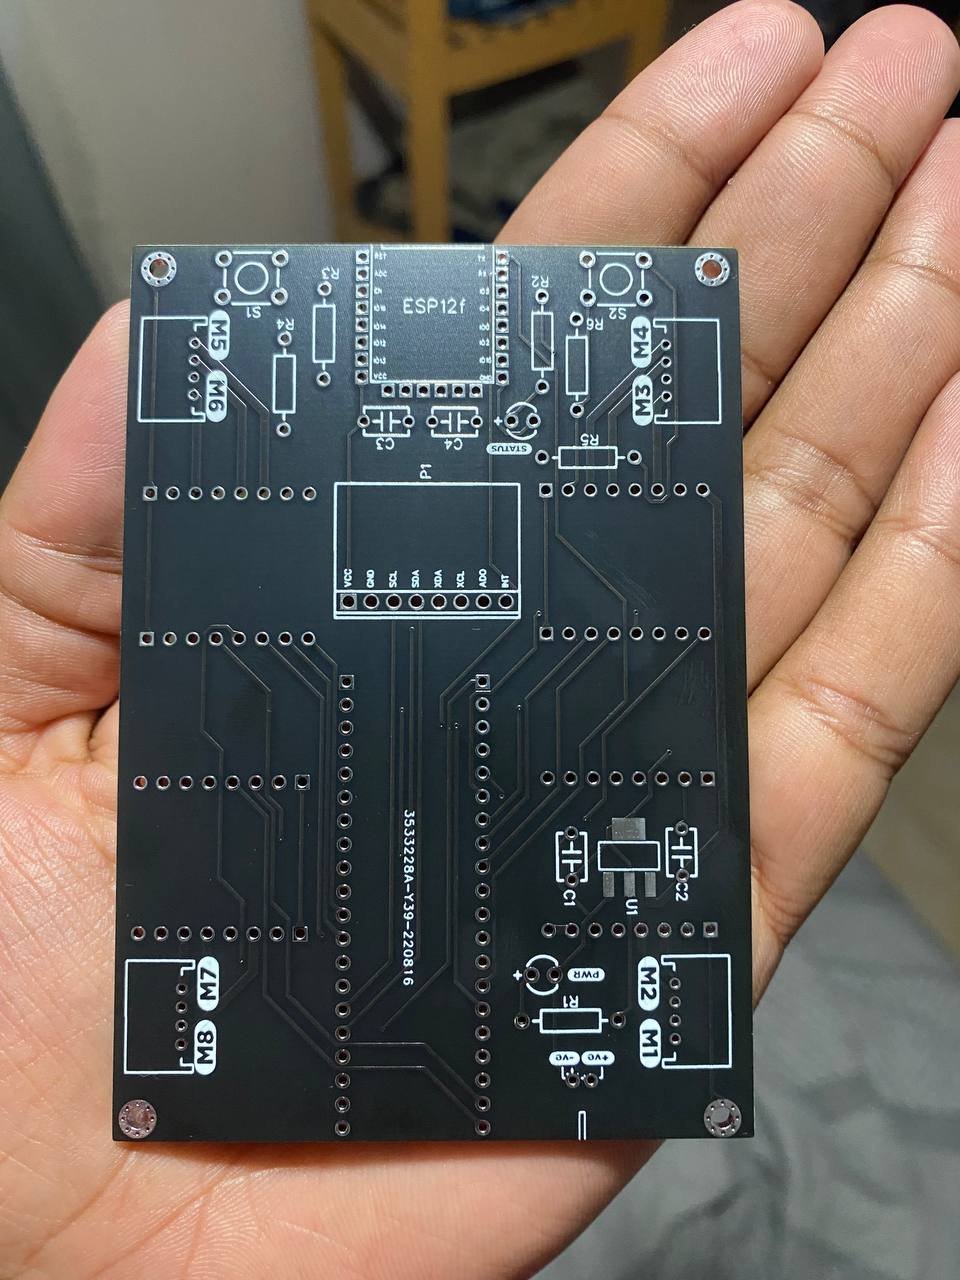
\includegraphics[scale = 0.25]{Figures/driverPCB.jpg}
    \caption{Main \ac{PCB}}
    \label{fig:PCB}
\end{figure}

Once the motor drivers, microcontroller and Wi-Fi client were acquired, they were assembled onto the main \ac{PCB} in Figure \ref{fig:PCB} to produce an assemblage of electronics shown in Figure \ref{fig:mainPCBAssembly}.

\begin{figure}[H]
\centering
    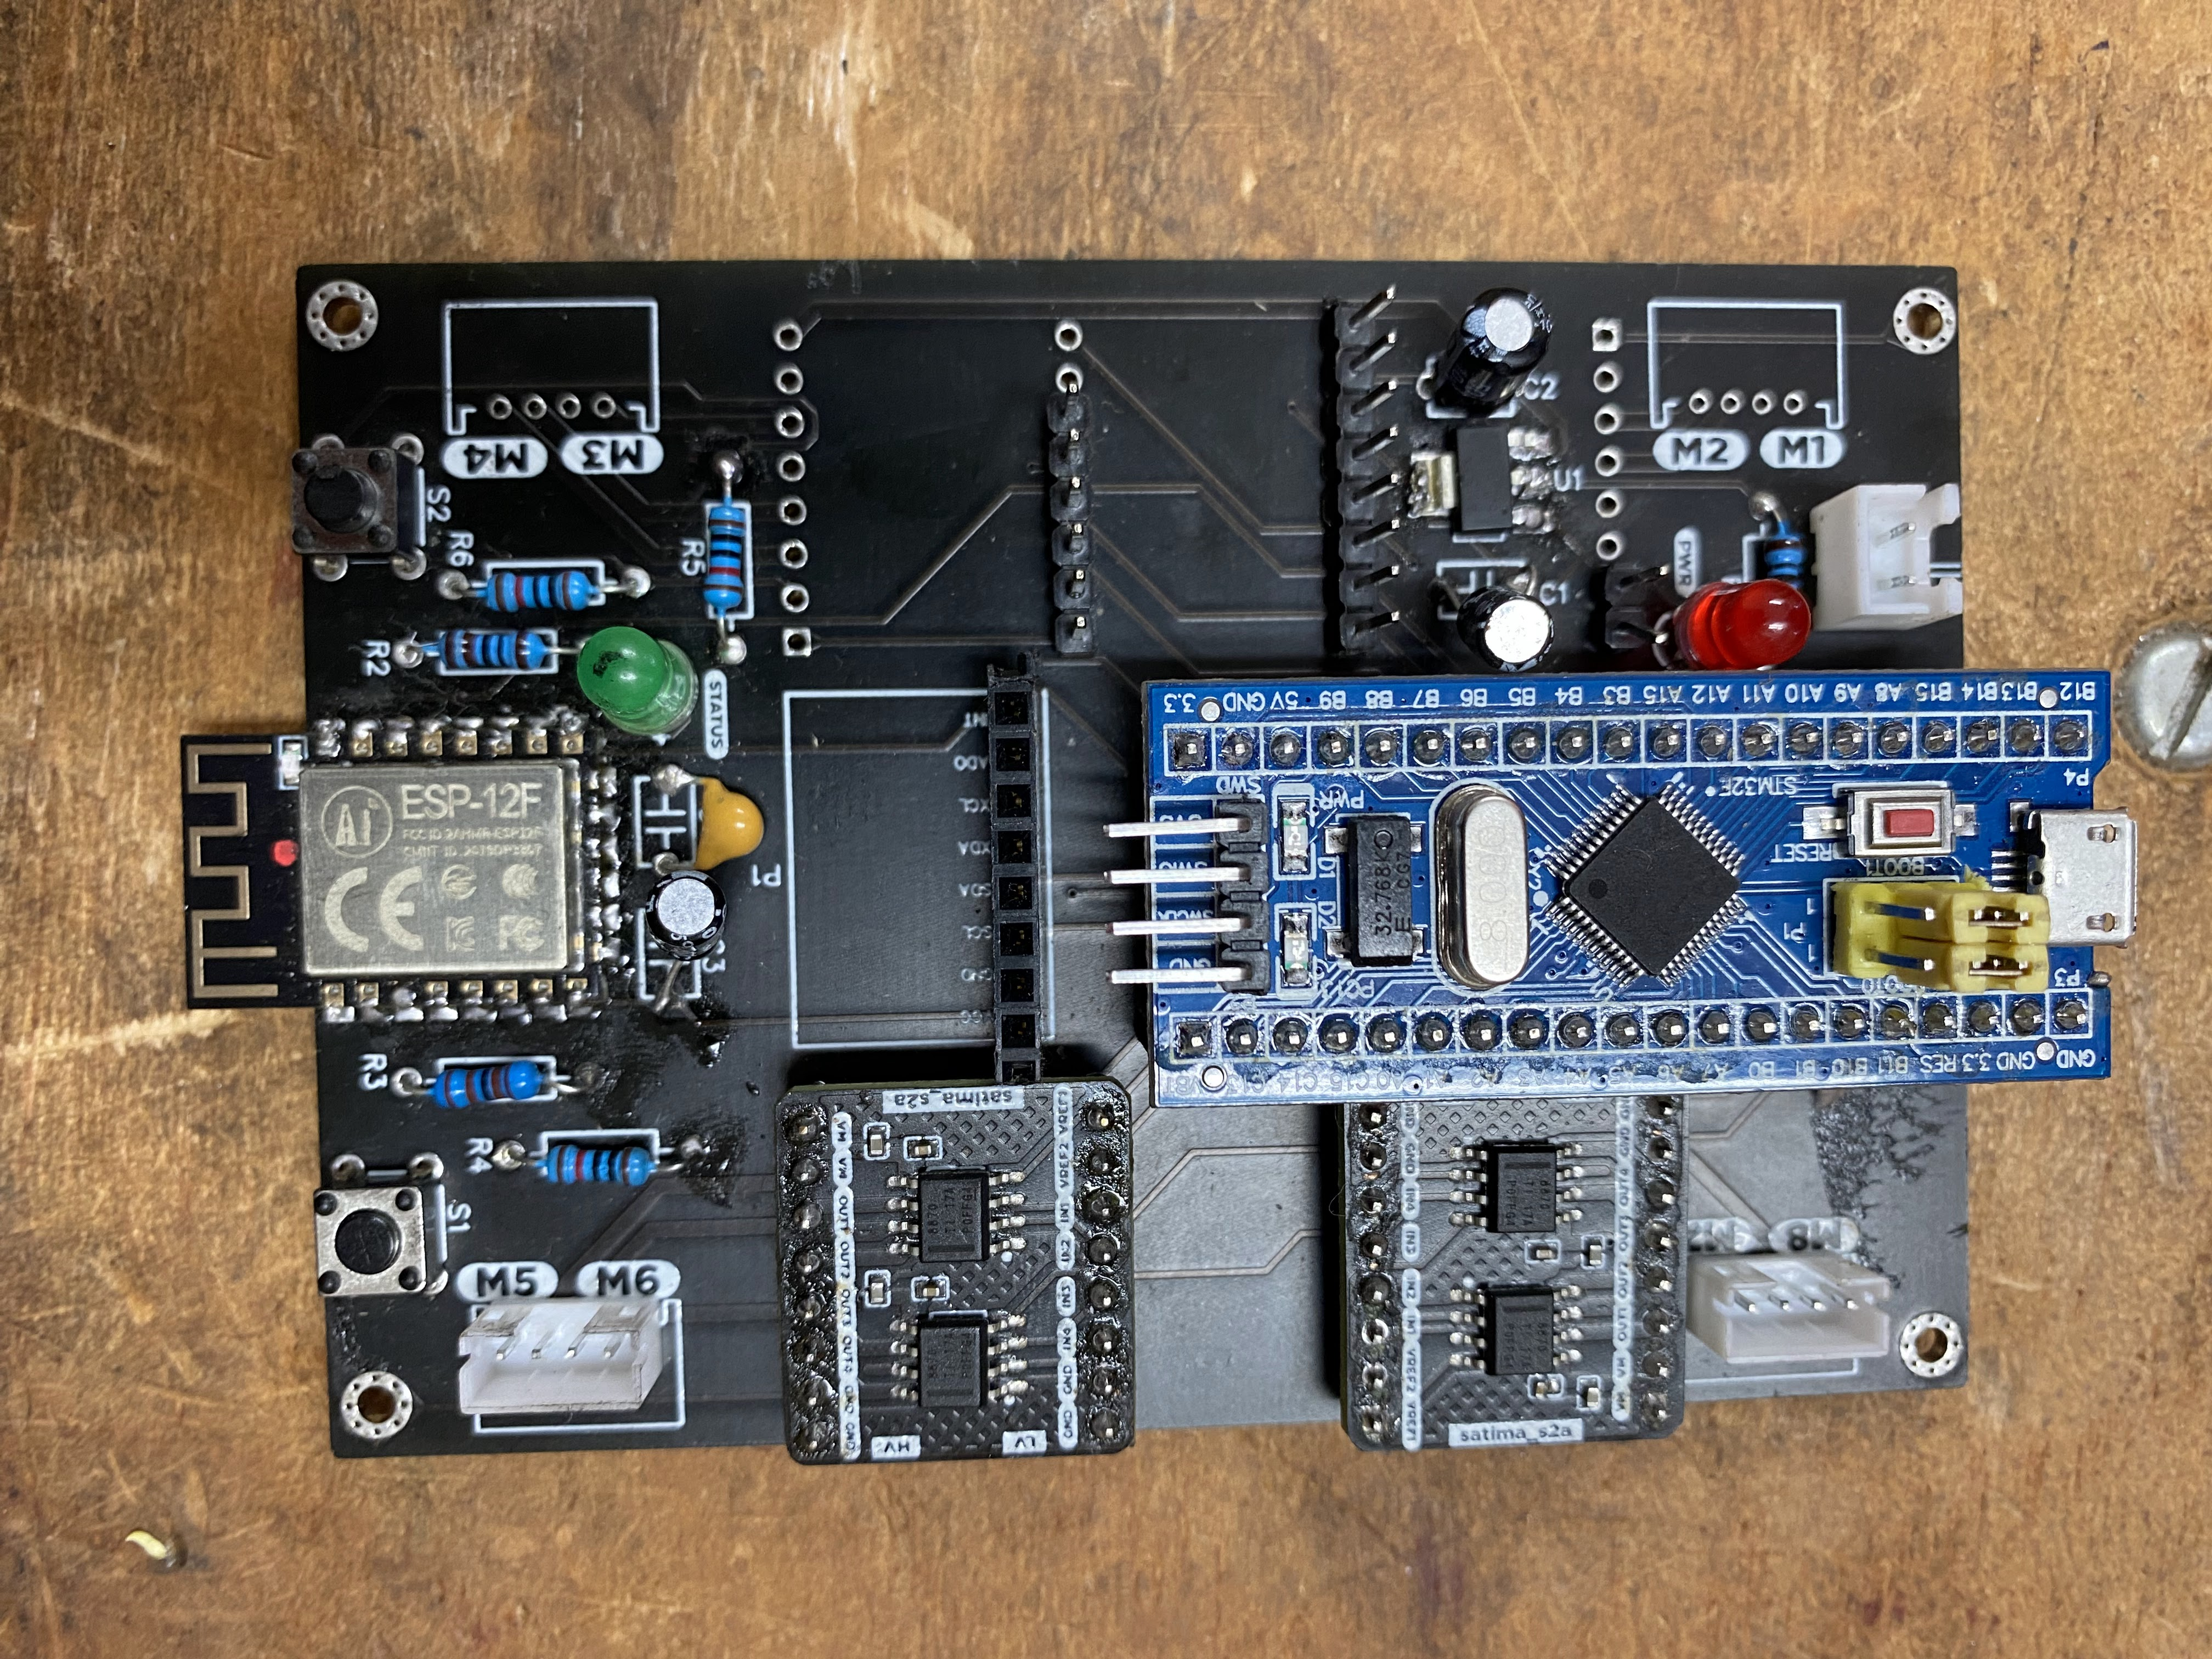
\includegraphics[scale = 0.07]{Figures/pcbFINALfront.jpg}
    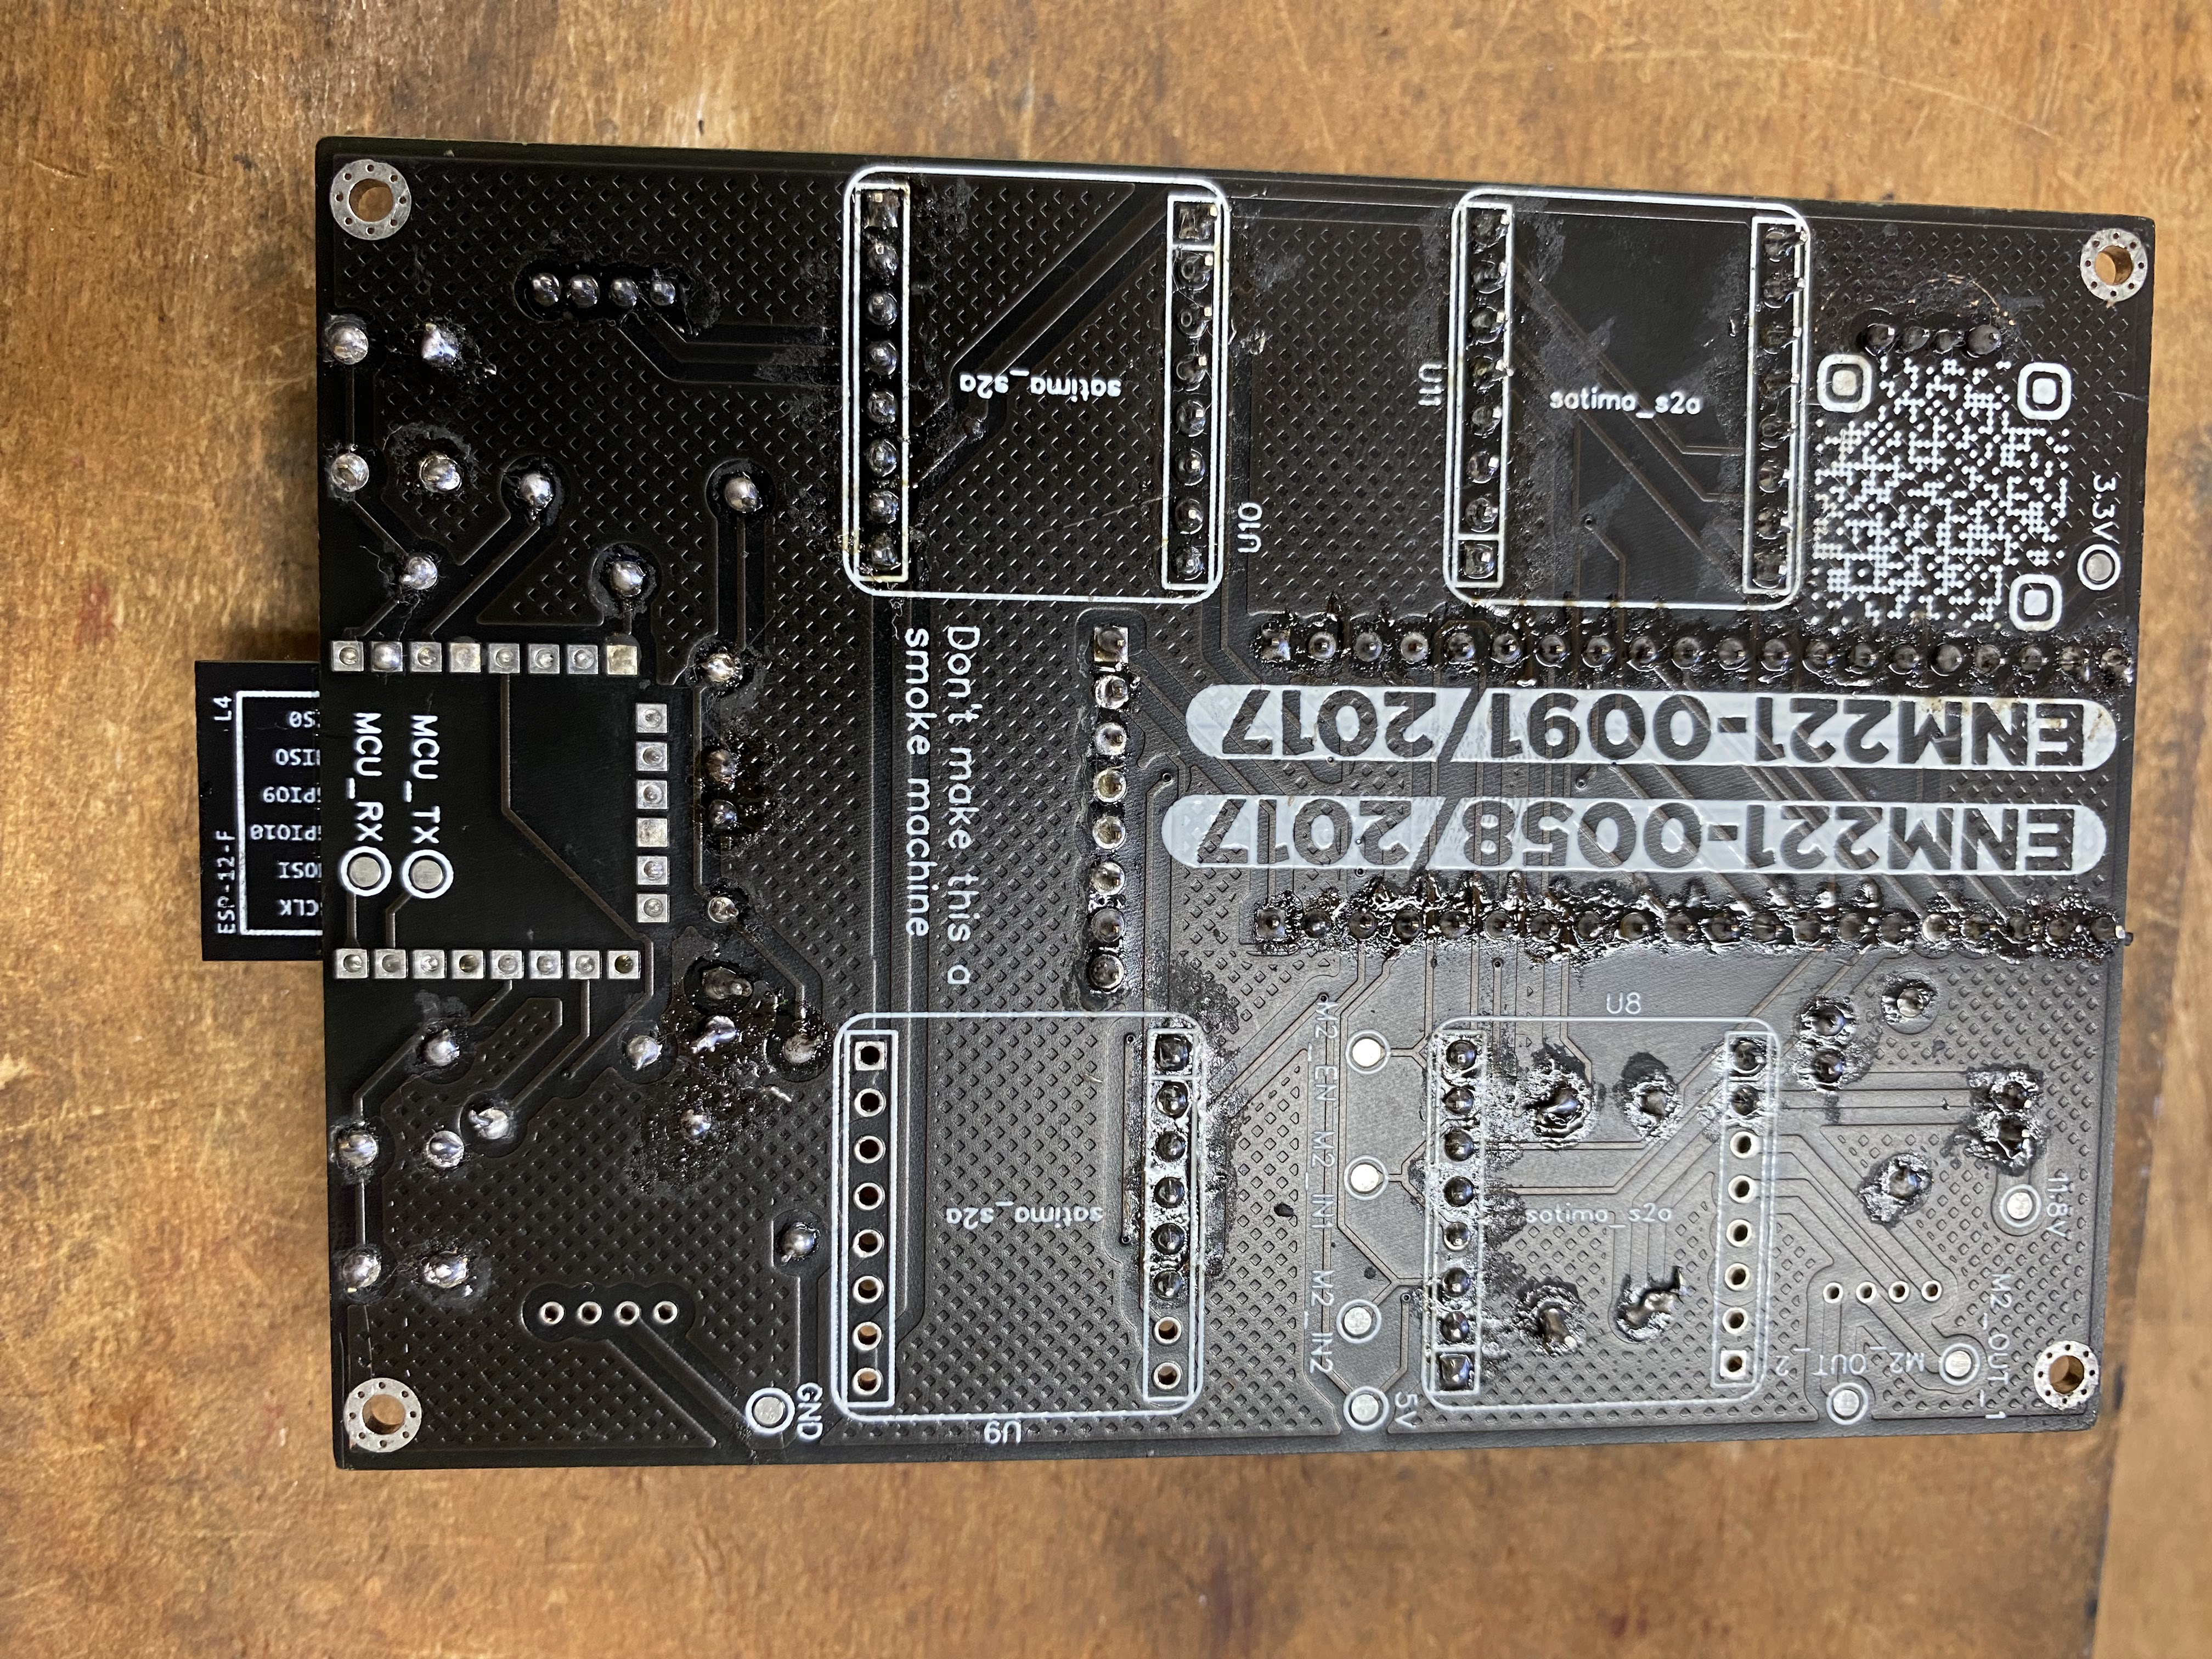
\includegraphics[scale = 0.07]{Figures/pcbFINALback.jpg}
    \caption{Platform \ac{PCB} Assembly}
    \label{fig:mainPCBAssembly}
\end{figure}

\par
In order to operate the mobile platform for at least an hour, a high capacity (greater than 900mAH) power source that can be recharged was the desired supply for the platform. Looking across the market, the 18650 Lithium Ion Battery 2200mAh 3.7V in Figure \ref{fig:lithiumBattery} was selected as most suitable for the job. This power supply was integrated into the main circuit as shown in Figure \ref{fig:mobileplatformmain}. 

\begin{figure}[H]
    \centering
    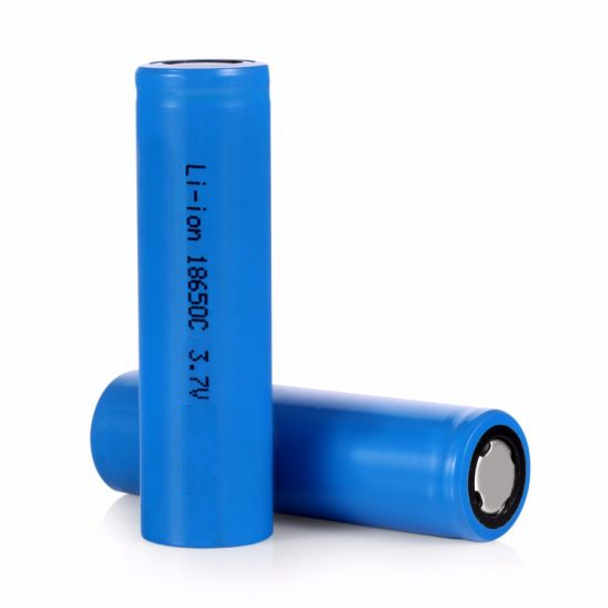
\includegraphics[scale = 0.3]{Figures/lithiumBattery.jpg}
    \caption{Lithium Ion Battery}
    \label{fig:lithiumBattery}
\end{figure}


\vspace{5mm}
For the sensory unit, the goal was to measure the acceleration and orientation of the mobile platform. For this, an \ac{IMU} was considered.
An \ac{IMU}, is an electronic device that measures and reports acceleration, orientation, angular rates, and other gravitational forces. It is composed of 3 accelerometers, 3 gyroscopes, and depending on the heading requirement – 3 magnetometers. That is to say, one per axis for each of the three vehicle axes: roll, pitch, and yaw.

There are different types of \ac{IMU} sensors \cite{noauthor_imu_nodate}: the one based on FOG (Fiber Optic Gyroscope), the RLG \ac{IMU}s (Ring Laser Gyroscope), and lastly, \ac{IMU} based on MEMS technology (Micro Electro-Mechanical Systems). This technology allows lower costs and low power requirements while ensuring performance. MEMS-based systems therefore combine high performance and ultra-low power in a smaller unit.
\par
The schematic developed for the sensory unit was used to incorporate the sensor into the other electronic components.

\begin{figure}[H]
    \centering
    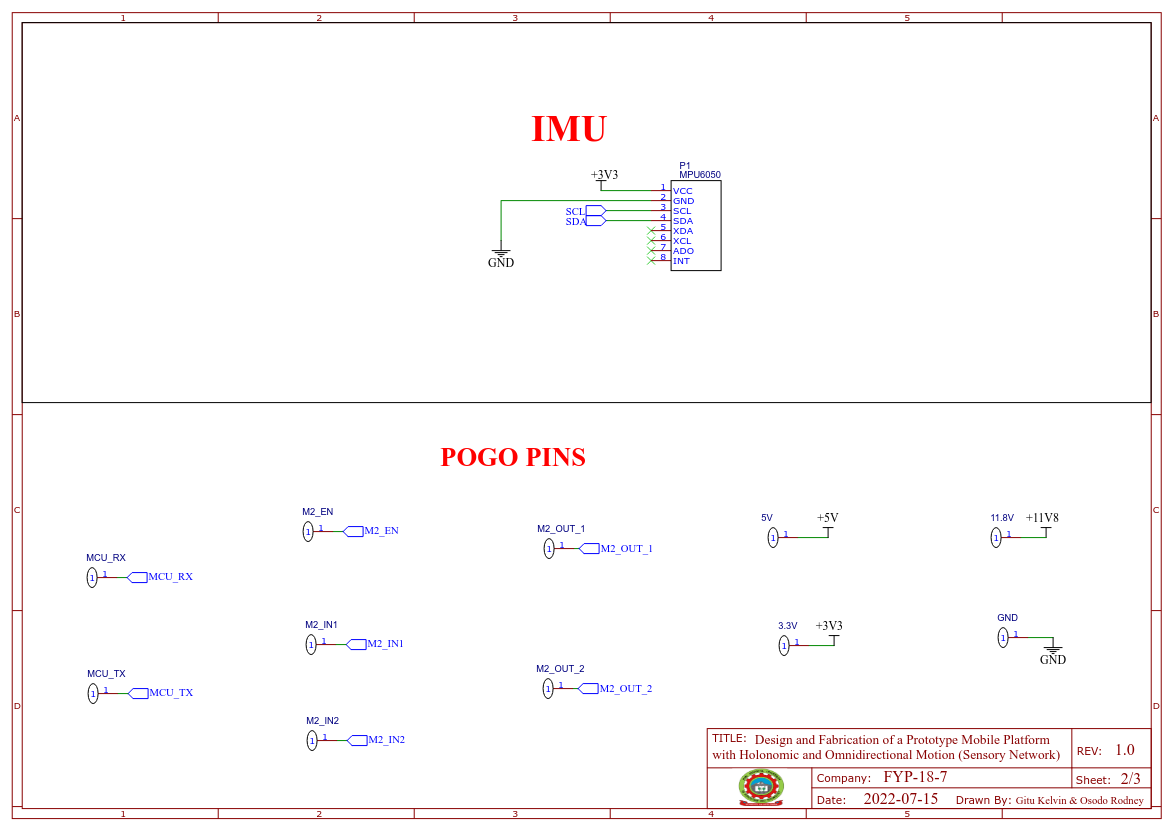
\includegraphics[scale=0.4]{Figures/MPsensory.png}
    \caption{Mobile Platform sensory schematic}
    \label{fig:mobileplatformsensory}
\end{figure}

\par
The \ac{IMU} selected for this particular application is the MPU6050 sensor module which is a complete 6-axis Motion Tracking Device. It combines 3-axis Gyroscope, 3-axis Accelerometer and Digital Motion Processor all in small package\cite{noauthor_mpu6050_nodate}. It also has additional feature of on-chip temperature sensor. This module is shown in Figure \ref{fig:mpu6050} and was acquired off-the-shelf. The number of modules that this application required were two. One was assembled onto the main platform \ac{PCB} in Figure \ref{fig:mainPCBAssembly} while the other was assembled onto the hand motion controller \ac{PCB} in Figure \ref{}.


\begin{figure}[H]
    \centering
    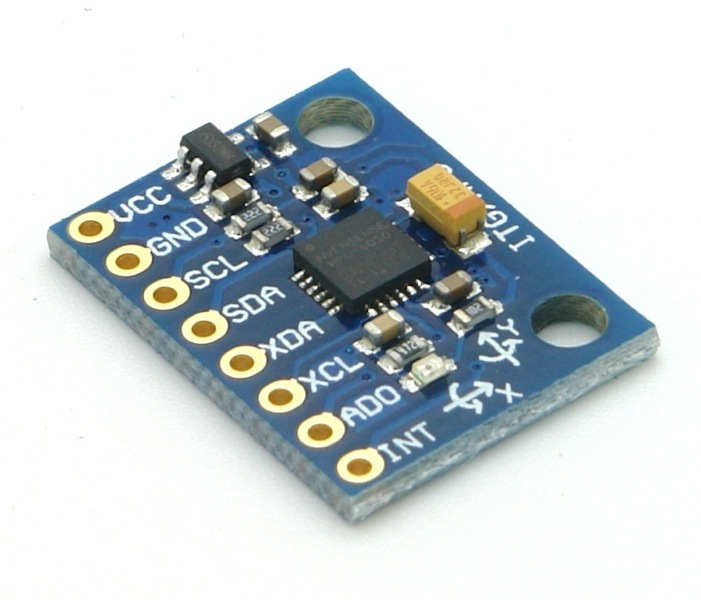
\includegraphics[scale=0.4]{Figures/MPU6050Module.jpg}
    \caption{MPU6050 Sensor Module}
    \label{fig:mpu6050}
\end{figure}

\subsection{Remote Control Clients}
\label{sec:remoteClients}

\subsubsection{Design}

\ac{API}s are code snippets that allow software applications to communicate in a common language. Web \ac{API}s enable client applications to access third-party data and seamlessly integrate it wherever and whenever it is needed, providing unrivalled data processing efficiencies and cost savings. 
\par
The goal of this project was to implement robot control using an \ac{API}. This would ensure integrating different clients as shown in Figure \ref{fig:omicronplatformcontrol}. 

More specifically, a mobile application and hand motion controller device would be the two control actions used for the platform.

\begin{figure}[H]
    \centering
    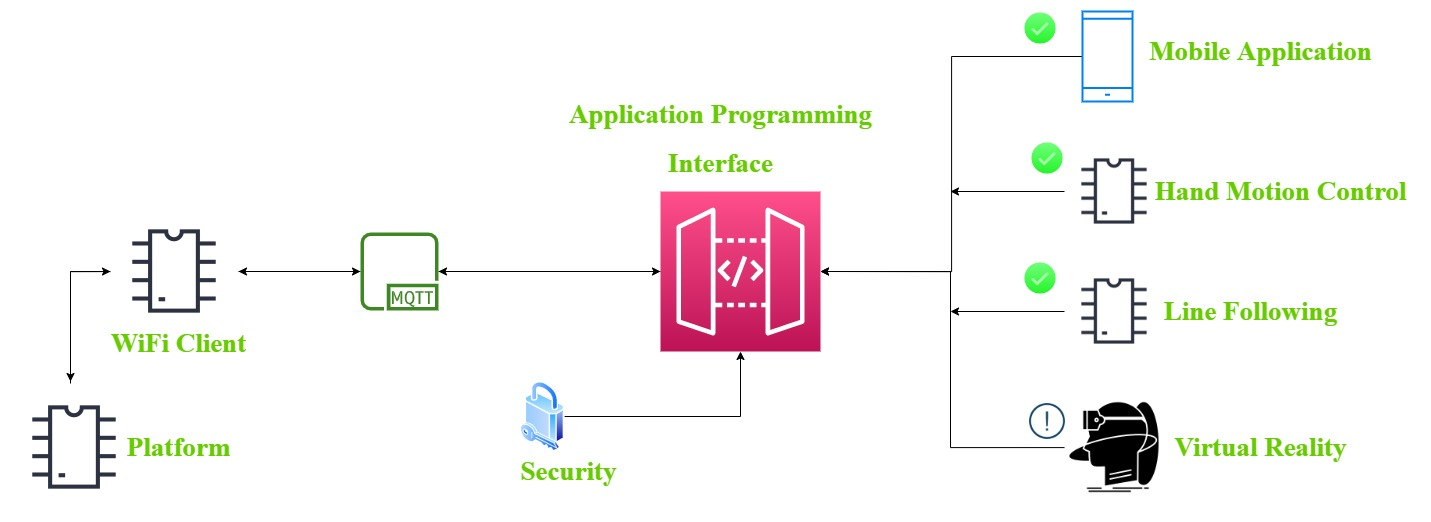
\includegraphics[scale=0.3]{Figures/omriconrobotPlatformControl.jpg}
    \caption{Mobile Platform Control Architecture}
    \label{fig:omicronplatformcontrol}
\end{figure}

\vspace{15mm}

The hand-motion controller is a hardware client that maps hand motions to actual commands that are sent to the mobile platform. The hand motion device is made up of an \ac{IMU} sensor in Figure \ref{fig:mpu6050} that would detect various hand motions. The \ac{CPU} interprets the motions and transmits the commands via a Wi-Fi client to the mobile platform microcontroller.

The schematic for the hand motion device in Figure \ref{fig:handmotionschematic} was developed using EasyEDA software. The main components of the device are the Wi-Fi client that also acts as the \ac{MCU}, power supply, a programmer, and the \ac{IMU} sensor.

\begin{figure}[H]
    \centering
    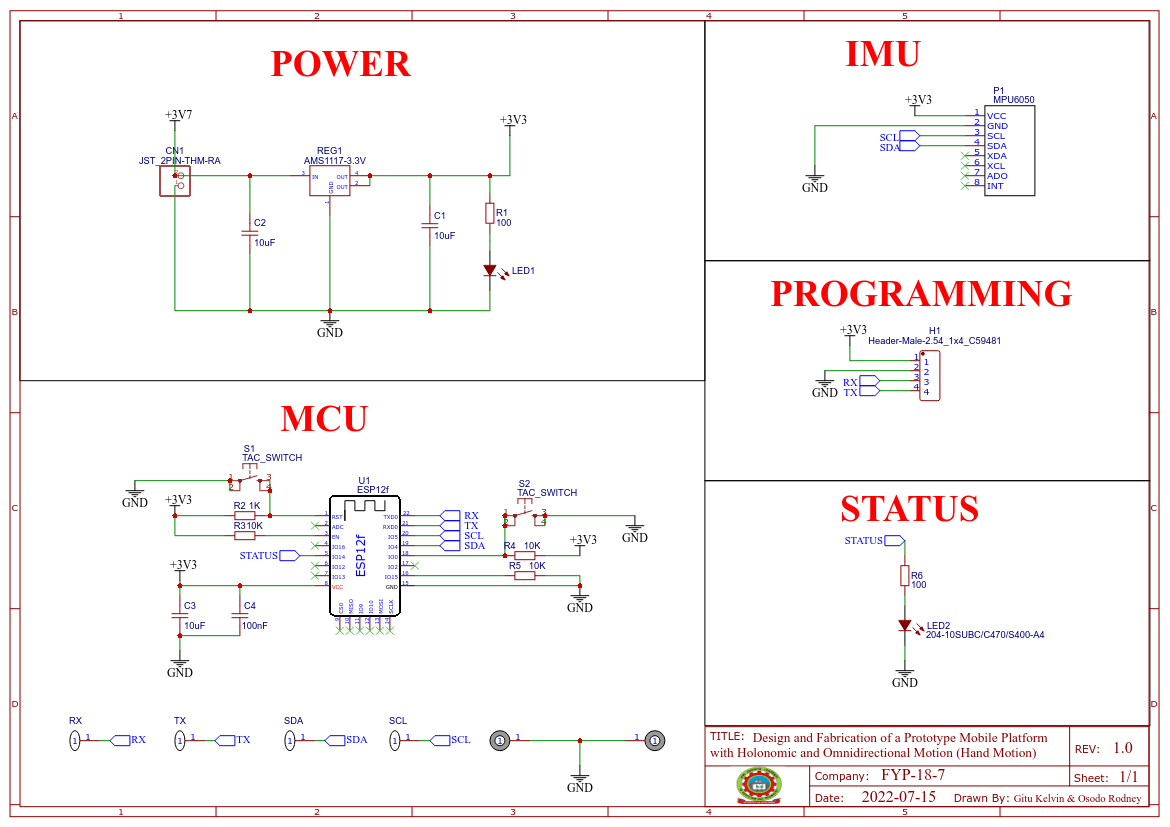
\includegraphics[scale=0.4]{Figures/HMSchematic.png}
    \caption{Hand Motion Schematic}
    \label{fig:handmotionschematic}
\end{figure}

For the mobile application client, software would be used to map inputs from the application to actual commands that would in turn be sent to the mobile platform. Several development tools were considered, including React native, Ionic, and Xamaric but ultimately Flutter seemed like the best platform for a number of reasons:
\begin{enumerate}[i.]
    \item Flutter used a simple implementation of the dart language which would be easy to learn and integrate
    \item Flutter could create multi-platform applications on a single code-base. That means applications that run on Android, Windows and iOS could be created using on code-base implementation.
    \item Flutter apps are relatively fast
\end{enumerate}

\subsubsection{Fabrication and Implementation}
With Mainflux, the robustness of our API is much increased. This is because, from our initial consideration, we wanted to build a multi protocol architecture. For instance, when we publish data using one protocol, we can receive it using another protocol. This is fundamental to increasing the robustness of our core API. Since we have different clients, we can either publish or subscribe data depending on the protocol that best suits the client.
\begin{enumerate}
    \item Mobile application - Web socket and \ac{HTTP}
    \item Hand motion controller - \ac{MQTT}
    \item Wifi Client - \ac{MQTT}    
\end{enumerate}

In this case, when we publish data using the mobile application using \ac{HTTP}, we can receive the same message using an \ac{MQTT} subscriber. \ac{MQTT} is a lightweight publish-subscribe messaging protocol that is commonly used in the \ac{IoT} for communication between devices.

In an \ac{IoT} system, \ac{MQTT} is used to establish a communication channel between devices, allowing them to exchange data and messages with each other. This allows devices to share information and coordinate their actions, enabling the \ac{IoT} system to function as a whole.

One of the key benefits of \ac{MQTT} is its low overhead and high efficiency. The protocol uses a simple and compact message format, which allows for efficient data transfer even over low-bandwidth or unreliable networks. This makes it well-suited for \ac{IoT} applications, where devices often have limited resources and may be connected through challenging networks.

Another advantage of \ac{MQTT} is its flexibility. The protocol supports different messaging patterns, such as publish-subscribe, request-response, and push-pull. This allows it to be used in a wide range of \ac{IoT} scenarios and applications, such as device-to-device communication, remote monitoring, and control.

Overall, \ac{MQTT} is an important component of the \ac{IoT} ecosystem, providing a reliable and efficient communication channel for devices to exchange data and messages.

Since we have three clients we create three things using the mainflux backend. These three things will be connected to one channel so that when the message is published to that channel any listening client can be able to receive the message. Mainflux provides support for both authorization and authentication.

Authorization refers to the process of determining whether a client has access to a certain resource or operation. In Mainflux, authorization is implemented using \ac{ACL} with the help of Keto as its main \ac{ACL} engine, which specifies the permissions that a client has to access a particular resource. For example, an \ac{ACL} may grant thing permission to read data from a specific channel or to control a particular device.

Authentication, on the other hand, refers to the process of verifying the identity of a thing. In Mainflux, authentication is implemented using \ac{JWT}, which are digitally signed tokens that contain information about the thing. When a thing attempts to access a resource, Mainflux verifies the \ac{JWT} to confirm its identity before granting access.

Overall, Mainflux provides support for both authorization and authentication to ensure that things are only able to access the resources and perform the operations that they are permitted to. This helps to protect the security and integrity of the \ac{IoT} system.
\par
The hand motion device was fabricated manually, which was different from other \ac{PCB}s as depicted in Sections \ref{sec:motorControl} and \ref{sec:platformControl}. The procedure for this process is described in detail in Section \ref{sec:PCBfab} and the result is depicted in Figure \ref{fig:handMotionPCB}.

\begin{figure}[H]
    \centering
    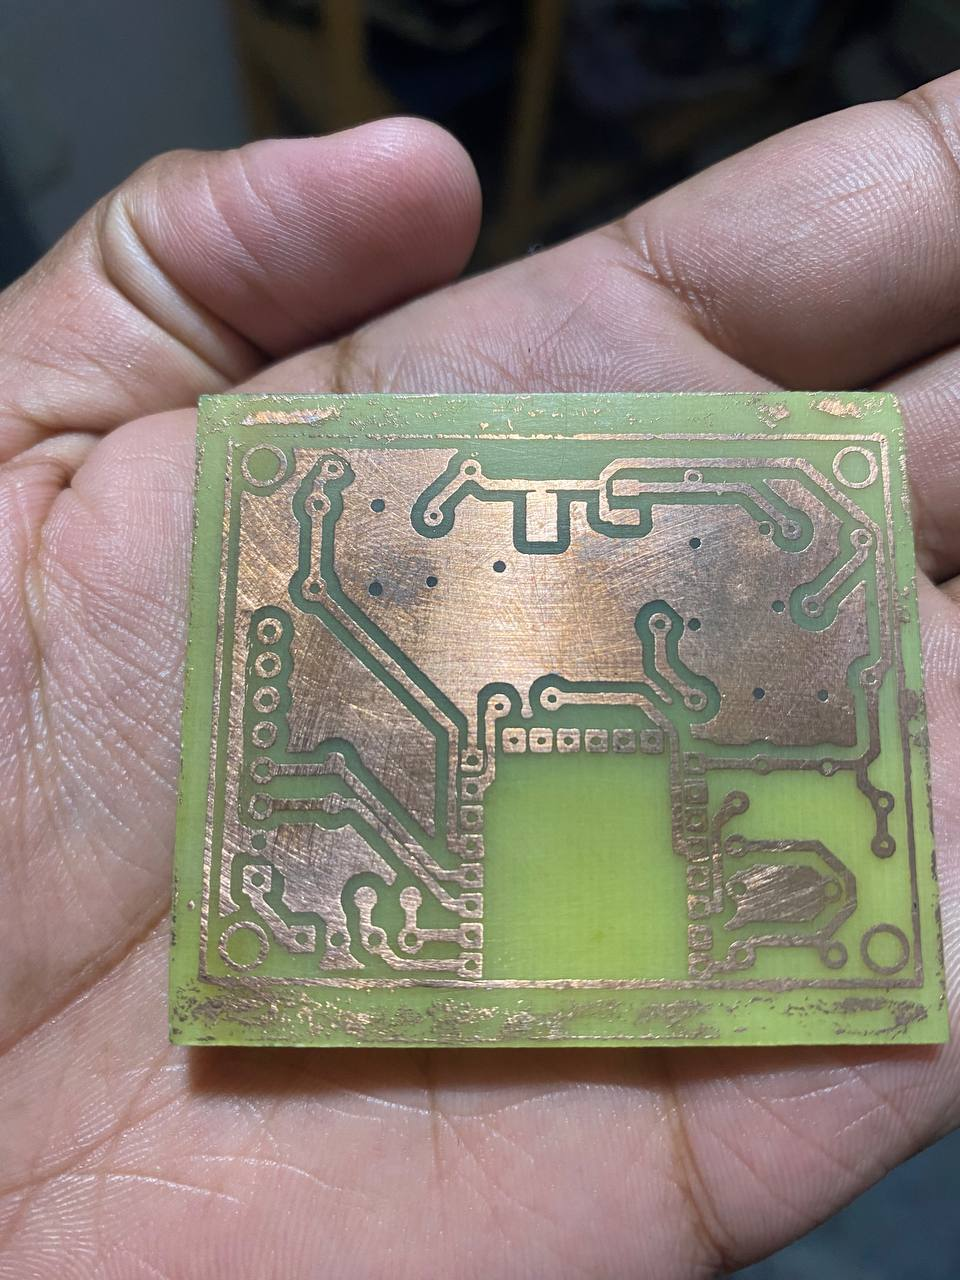
\includegraphics[scale = 0.2]{Figures/handMotionPCB.jpg}
    \caption{Hand Motion Device \ac{PCB}}
    \label{fig:handMotionPCB}
\end{figure}

The Wi-Fi client, \ac{IMU} sensor and other components were soldered onto the hand motion device \ac{PCB} using a soldering gun and wire.

\begin{figure}[H]
    \centering
    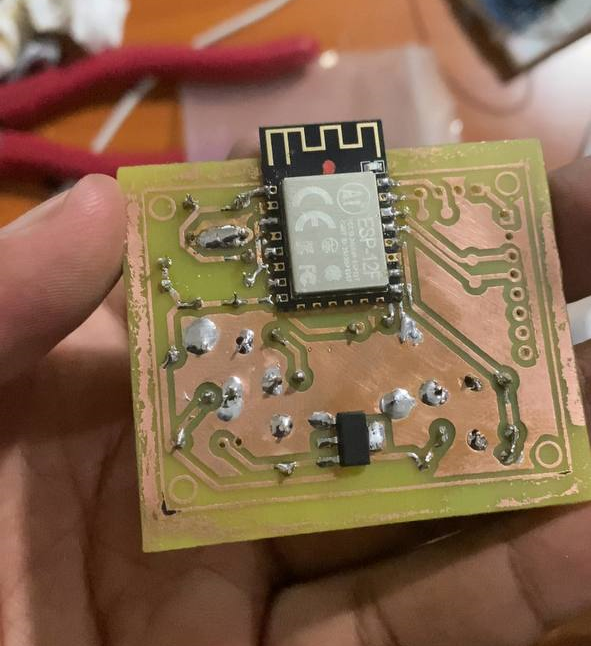
\includegraphics[scale = 0.4]{Figures/handMotionFront.png}
    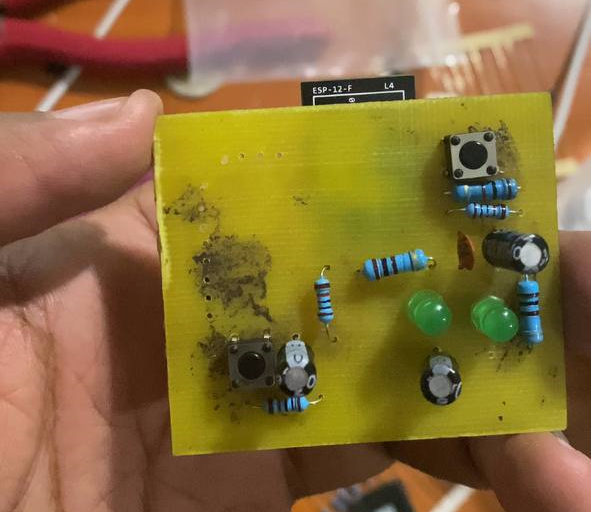
\includegraphics[scale = 0.4]{Figures/handMotionBack.png}
    \caption{Assembled Hand Motion Device \ac{PCB}}
    \label{fig:handMotionAssembly}
\end{figure}

For the mobile application, implementation was done using various software tools. A code editor, Visual Studio Code was used to write dart code for the application. Another editor, Android Studio provided an emulator on which to edit the application in real-time. This ensured that any changes could be seen during active development. Flutter's official documentation was used as a guide, especially where challenges arose. Figure \ref{fig:flutterPages} is a representation of some of the pages that were developed using the code in Section \ref{sec:code}

\begin{figure}[H]
    \centering
    
\includegraphics[scale = 0.2]{Figures/flutterOne.jpg}
    
\includegraphics[scale = 0.2]{Figures/flutterTwo.jpg}
    
\includegraphics[scale = 0.2]{Figures/flutterThree.jpg}
    \caption{Flutter App Pages}
    \label{fig:flutterPages}
\end{figure}









